\documentclass[a4paper, portrait,12pt]{report}
%\usepackage[scaled]{helvet}
\renewcommand\familydefault{\sfdefault} 
\usepackage[T1]{fontenc}
\usepackage[verbose,a4paper,tmargin=2.5cm,bmargin=2.5cm,lmargin=2.5cm,rmargin=2.5cm]{geometry}
\usepackage[utf8]{inputenc}
\usepackage{polski}
\usepackage{amsmath}
\usepackage{amsfonts}
\usepackage{amssymb}
\usepackage{lastpage}
\usepackage{indentfirst}
\usepackage{float}
\usepackage{verbatim}
\usepackage{graphicx}
\usepackage{fancyhdr}
\usepackage{multirow}
\usepackage{array}
\usepackage{multicol}
\usepackage{tabu}
\usepackage{fancyhdr}
\usepackage{enumitem}
\pagestyle{fancy}
\frenchspacing
\pagestyle{fancyplain}
\fancyhf{}
\renewcommand{\headrulewidth}{0pt}
\renewcommand{\footrulewidth}{0.4pt}
\newcommand{\degree}{\ensuremath{^{\circ}}} 
\fancyhead[L]{WYDZIAŁ FIZYKI TECHNICZNEJ, INFORMATYKI i MATEMATYKI STOSOWANEJ \\
Instytut Fizyki PŁ}
\lhead{\small WYDZIAŁ FIZYKI TECHNICZNEJ, INFORMATYKI i MATEMATYKI STOSOWANEJ \\ Instytut Fizyki PŁ,}
\fancyfoot[C]{\thepage}
\renewcommand{\headrulewidth}{0.4pt}
\renewcommand{\footrulewidth}{0.4pt}
\newcolumntype{C}[1]{>{\centering\let\newline\\\arraybackslash\hspace{0pt}}m{#1}}
\setcounter{page}{1}
\usepackage{listings}
\usepackage{color}
 
\definecolor{codegreen}{rgb}{0,0.6,0}
\definecolor{codegray}{rgb}{0.5,0.5,0.5}
\definecolor{codepurple}{rgb}{0.58,0,0.82}
\definecolor{backcolour}{rgb}{0.95,0.95,0.92}
 
\lstdefinestyle{mystyle}{
    backgroundcolor=\color{backcolour},   
    commentstyle=\color{codegreen},
    keywordstyle=\color{magenta},
    numberstyle=\tiny\color{codegray},
    stringstyle=\color{codepurple},
    basicstyle=\footnotesize,
    breakatwhitespace=false,         
    breaklines=true,                 
    captionpos=b,                    
    keepspaces=true,                 
    numbers=left,                    
    numbersep=5pt,                  
    showspaces=false,                
    showstringspaces=false,
    showtabs=false,                  
    tabsize=2
}
 
\lstset{style=mystyle}


\usepackage{xcolor}
\lstset { %
    language=C++,
    backgroundcolor=\color{black!5}, % set backgroundcolor
    basicstyle=\footnotesize,% basic font setting
}


\begin{document}
\tableofcontents    % generuje spis treści ze stronami !!! 
\newpage

\chapter{Wstęp} \label{rozdz.wstep}
Niniejsza praca dotyczy zakresu inżynierii oprogramowania sprzętu pomiarowego w celu wykorzystania go w badaniu charakterystyk laserów półprzewodnikowych w laboratorium fotoniki Politechniki Łódzkiej. \\

Głównym celem pracy jest przedstawienie wykorzystania systemu Linux oraz oprogramowania open source w badaniach naukowych na przykładzie stworzenia interfejsu
pomiarowego w laboratorium fononiki do badania charakterystyk laserów półprzewodnikowych. \\

W ostatnich latach obserwuje się gwałtowny rozwój wykorzystania oprogramowania
open source w codziennej pracy naukowej. Coraz większą popularność zdobywa język Python. Od dawana podstawowym systemem operacyjnym używanym przez naukowców są różne odmiany systemu Unix. Jest to spowodowane dostępnością wielu narzędzi (C, Python,
Gnuplot) których naturalnym środowiskiem jest środowisko Linux, ułatwiającym pracę naukową. Inną
zaletą środowiska Unix jest możliwością korzystanie z linii poleceń, która ułatwia wiele
zadań. Szukając informacji o wykorzystaniu języka Python do komunikacji ze sprzętem pomiarowym można zauważyć pewną lukę, którą moja praca ma cel wypełnić. Korzystając
z strony oraz dokumentacji firmy Thorlabs, której sprzęt jest używany w laboratorium
fononiki, należy zauważyć brak programu do komunikacji ze sprzętem na platformie Linux.
Dostępne są jedynie wysokopoziomowe API do systemu Windows oraz możliwość użycia
LabVIEW. Minusów środowiska Windows nie sposób wymienić w kilku zdaniach. Program
LabVIEW jest programem płatnym. Rozwiązaniem wszystkich problemów jest użycie środowiska Linux, gdzie wszystko jest plikiem, także sprzęt połączony przez usb z komputerem, dzięki czemu możemy się z nim komunikować używając standardu komend SCPI przez
wykorzystanie wywołań systemowych. Dzięki temu mamy możliwość dostępu do wszystkich możliwych funkcji sprzętu pomiarowego bez ponoszenie kosztów. Umożliwia nam to
sterowania sprzętu za pomocą komputera oraz wizualizacje i analizę danych w sposób, jaki
potrzebujemy. A wszystko to dzięki połączeniu możliwości środowiska Linux oraz języka Python \\

Głównymi celem mojej pracy jest przedstawienie wykorzystanie oprogramowania
open source takiego jak Python, C/C++ oraz systemu Linux do stworzenia stanowiska pomiarowego w celu bdania laserów półprzewodnikowych. Korzystając z tych technologi mam zamiar stworzyć interfejs pomiarowy na platformę Ubuntu
w laboratorium fotoniki. \\
Dzięki mojej pracy możliwe będzie wykonywanie w szybki sposób charakterystyk laserów półprzewnodnikowcyh. Charakterystyki te dają nam ważne informacje o laserze, dzięki nim możliwe jest określenie prądu progowego dla laserów krawędziowych, określenie ich sprawności. Za pomocą mojego stanowiska pomiarowego możliwe także będzie badanie ile uzyskuje się mocy z lasera przy danej mocy aplikowanej. \\
Praca jest podzielona na dwie części: jedna składa się z opisu przygotowania eksperymentu, komunikacji oraz sterowaniem urządzeniami laboratoryjnymi za pomocą programu napisanego w języku Python. Druga część pracy opisuje badanie laserów półprzewodnikowych na podstawie danych uzyskanych za pomocą programu przedstawionego w pierwszej części programu. Do wykreślenia charakterystyk wyjściowych oraz wyznaczenie sprawności badanych laserów używam skryptów napisanych w języku Python.



\chapter{Komunikacja z urządzeniami pomiarowymi na platformie Linux}
\section{Programowane urządzenia pomiarowe}
Przez  programowane urządzenia pomiarowe rozumiemy sprzęt mogący dokonywać pomiarów wielkości elektrycznych i nieelektrycznych, który wyposzażony jest w interfejs umożliwiający sterowanie nimi przy pomocy komputera. Przykładami takich urządzeń, którymi zajmuje się w swojej pracy są:
\begin{itemize}
\item Zasilacza diód laserowych firmy Thorlabs model LDC4005.
\item Miernik mocy firmy Thorlas firmy Thorlabs model PM100.
\end{itemize}
Z wyżej wymienionymi urządzeniami możliwa jest fizyczna komunikacja za pomocą interfejsu USB przy pomocy standardu komend SCPI, który zostanie opiszany w dalszej cześci rozdziału.

\section{Komunikacja}
W systemach Unix z którego dziedziczy system Linux, wszystko jest plikiem. Linuksowy sterownik znakowy (ang. \textit{char driver}) pozwala na reprezentowanie urządzenia za pomocą specjalnych plików wirtualnych, które znajdują się w przestrzeni użytkownika w katalogu $\mathtt{/dev/<nazwa>}$. Obsługa tych plików możliwa jest za pomocą wywołań systemowych (ang. \textit{system call}), które stanowią API za pomocą którego użytkowniki może sterować sprzętem. Podstawowe wywołaniami systemowymi pozwalające na sterowanie sprzętem to:
\begin{itemize}
\item $\mathtt{open}$ --- służy do połaczenia z urządzeniem, zwraca deskrypotor pliku.
\item $\mathtt{write}$ --- funkcja służaca do wysyłania komend do urządzenia .
\item $\mathtt{read}$ --- funckja służąca do odczytywania buffora urządzenia.
\item $\mathtt{close}$ --- funkcja zamykająca połączenie.
\end{itemize}
Funckje te mają swoją implementacje w języku C w bibliotecze $<\mathtt{fcntl.h}>$, oraz w języku Python w bibliotecze $\mathtt{os}$.
\section{SCPI --- standard komend do komunikacji z urządzeniami}
SCPI  (ang. \textit{Standard  Commands  for  Programmable  Instruments}) jest tekstowym interfejsem ASCII do programowanych urządzeń pomiarowych mający na celu standaryzacje polecenie używanych w systemach pomiarowym. Zdefiniowany został 1990 roku, wedle specyfikacji IEEE 488.2. (Institute of Electrical and Electronics Engineers, międzynarodowa organizacja stowarzyszeń inżynierów elektryków i elektroników.  Dzięki temu możliwa jest obsługa tych urządzeń przy wykorzystaniu komputera. Polecenia SCPI są to ciągi tekstowe ASCII, które są wysyłane do urządzenia. Polecenia są serią jednego lub więcej słów, przy czym wiele z nich używa dodatkowych parametrów. Odpowiedzi do zapytania polecenia są zazwyczaj ciągami ASCII. W przypadku danych masowych mogą być użytawane także formaty binarne. \\

Cechą  poleceń  wspólnych  (ang.  common)  jest  ich  implementacja  przez  każde urządzenie. Czyli naprzykład to samo polecenie będzie działać na każdym oscyloskopie bez względu na producenta. Można wyróżnić dwie grupy poleceń:
\begin{itemize}
\item Polecenia dla każdego urządzenia pomiarowego nie zależnie od jego przeznacznia. Takimi komendami są m.in.
\begin{itemize}
\item $\mathtt{*idn?}$ --- odczytuje identyfikator urządzenia. 
\item $\mathtt{*rst}$ --- powduje przywrócenie ustawień początkowych urządzenia.
\item $\mathtt{*cls}$ --- powduje wyzerowanie informacji o błędach.
\item $\mathtt{*opc?}$  --- (ang.  operation  complete)  zapytanie  o  zakończenie  wykonania
poprzedzających poleceń. \\
W  odpowiedzi  na  zapytanie  po  zakończeniu  wykonywania  poprzedzających poleceń urządzenie prześle wartość 1.
\item $\mathtt{*wai}$ ---  (ang.  wait)  oczekiwanie  na  zakończenie  wykonania  poprzedzających poleceń.
\end{itemize}

\item Polecenia charakterystyczne dla danego urządzenia pomiarowego zgodnie z jego przeznaczeniem. Przykładowe polecenie które będzie działać na każdym zasilaczu korzystającym z standardu SCPI:
\begin{itemize}
\item Służacę do ustawienie wartości prądu na 0.01\,A \\ $\mathtt{SOURce:CURRent:LEVel:AMPLitude}$  $\mathtt{0.01}$
\end{itemize}
\end{itemize}

Fizyczne łącze komunikacyjne nie jest zdefiniowane przez SCPI. Stworzony standard IEEE-488 był dla GPIB, ale może być również używany z interfejsem RS-232, Ethernet, USB, VXIbus.
\newpage
\section{Przykładowe programy do sterowania sprzętem}
Przykładowy program w języku Python do zapytania sprzętu o jego nazwe.
\lstinputlisting[language=Python, firstline=0, lastline=20]{deviceio.py}
Przykładowy program w języku C do zapytania sprzętu o jego nazwe.
\begin{lstlisting}
#include<errno.h>
#include<fcnl.h>
#include<unistd.h>
#include<stdio.h>

int main()
{
    int fd = open("/dev/usbtmc0", O_RDWR | O_NOCTTY);
    if(fd == -1) {
        perror("open");
        exit(EXIT_FAILURE);
    } else {
        write(fd, "*IDN?", 100);
        char buffor[128];
        read(fd, buffor, 128);
        printf(buffor);
    }
}

\end{lstlisting}

\newpage

\chapter{Py3LabDeviceIO --- moduł do sterowania sprzetem laboratoryjnym}
\section{Opisz programu}
PyLabDeviceIO jest modułem napisanym w języku Python umożliwającym sterowanie zasilaczem do lasera oraz miernikiem mocy. Program opiera się na wykorzystaniu wywołań systemowych oraz na komunikacji przez komendy SCPI. \\

Program składa sie z czterech klas:
\begin{itemize}
\item $\mathtt{device.py}$ --- główna klasa, zawiera funkcje: do sprawdzania dostępnych urządzeń, 
zwraca instancje danego urządzenia, co umażliwa korzystanie z jego funkcji. 
\item $\mathtt{IODevice.py}$ --- klasa do operacji wejścia-wyjścia na programowalnych urządzeniach pomiarowych.
\item $\mathtt{LDC4005.py}$ --- klasa zawierająca funkcje od obsługi zasilacza diód laserowych Thorlabs 4005.
\item $\mathtt{PM100.py}$ --- klasa zawierająca funkcje do obsługi detektora mocy Thorlabs PM100.
\end{itemize}
\begin{figure}[h]
\center
  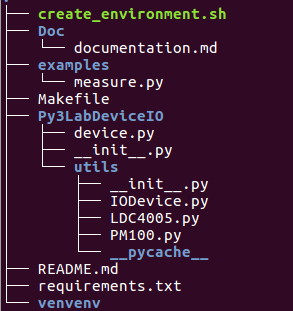
\includegraphics[scale=0.45]{tree.png}
  \label{rys1}
  \caption{Strukura programu.} 
\end{figure}
\section{Używanie programu}
W celu dokonania pomiarów za pomocą programu Py3LabDeviceIO możliwe są dwie operacje:
\begin{itemize}
\item wywołanie skryptu z linii poleceń z odpowienimi parametrami.
\item uruchomienie programu okienkowego.
\end{itemize}
Obie wymagają uprawnień użytkownika uprzywijowanego (sudo).
\newpage
\chapter{Gui}
\section{Gui}
\begin{figure}[h]
\center
  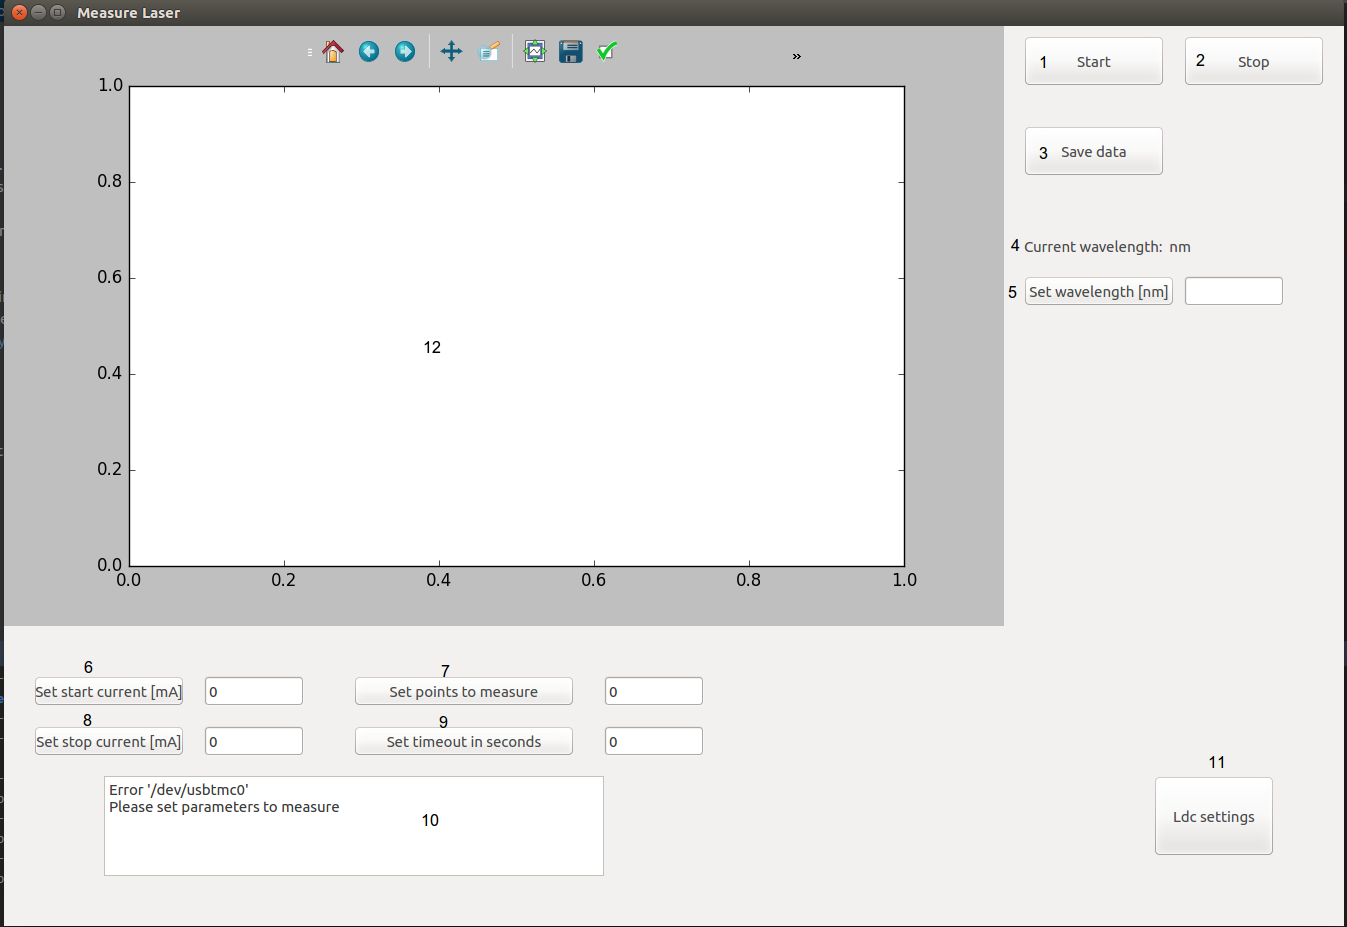
\includegraphics[scale=0.35]{gui.png}
  \label{rys1}
  \caption{1 --- rozpoczecie pomiarów, 2 --- zatrzymanie pomiarów, 3 --- zapisanie danych pomiarowych, 4 --- pokazuje długość fali detektora, 5 --- zmiana długości fali detektora.} 
\end{figure}
\chapter{Eksperyment} \label{Eksperyment}
\section{Teoria}
\subsection{Prąd progowy}
Wśród laserów półprzewodnikowych możemy wyróżnić lasery krawędziowe oraz lasery o emisji powierzchniowej z pionową wnęką rezonansową tzw. Lasery VCSEL (ang. \textit{Vertical Cavity Surface Emitting Laser}) będące obiektem moich badań. Aby scharakteryzować lasery, można wykonać ich charakterystyki, które przedstawiają, jak zmienia się moc wyjściowa oraz napięcie lasera w funkcji zadanego prądu.

Ważnym parametrem laserów półprzewodnikowych jest prąd progowy (z ang. \textit{threshold
current}) który określa wartość prądu, przy którym zaczyna zachodzić akcja laserowa, czyli
rośnie gwałtownie natężenie promieniowania i maleje szerokość linii emisyjnej. W celu wyznaczenia prądu progowego należy sporządzić wykres zależności mocy wyjściowej lasera od prądu zasilającego. Następnie dla prądu gdzie zaczyna się akcja laserowa dla odcinka liniowego należy metodą najmniejszych kwadratów przy użyciu wielomianu pierwszego stopnia znaleźć parametry krzywej. Dla wyznaczonej krzywej należy znaleźć miejsce zerowe, które będzie wyznaczonym prądem progowym.
\begin{equation}
P = a \cdot I + b
\end{equation}
\begin{equation}
I_{th} = -\frac{b}{a}
\end{equation}
\begin{equation}
\Delta I_{th} = \left\lvert \frac{\partial I_{th}}{\partial a} \right\rvert \cdot \Delta a + \left\lvert \frac{\partial I_{th}}{\partial b} \right\rvert \cdot \Delta b
\end{equation}
\begin{equation}
\Delta I_{th} = \left\lvert -\frac{b}{a^2} \right\rvert \cdot \Delta a + \left\lvert -\frac{1}{a} \right\rvert \cdot \Delta b 
\end{equation}
\begin{figure}
\center
  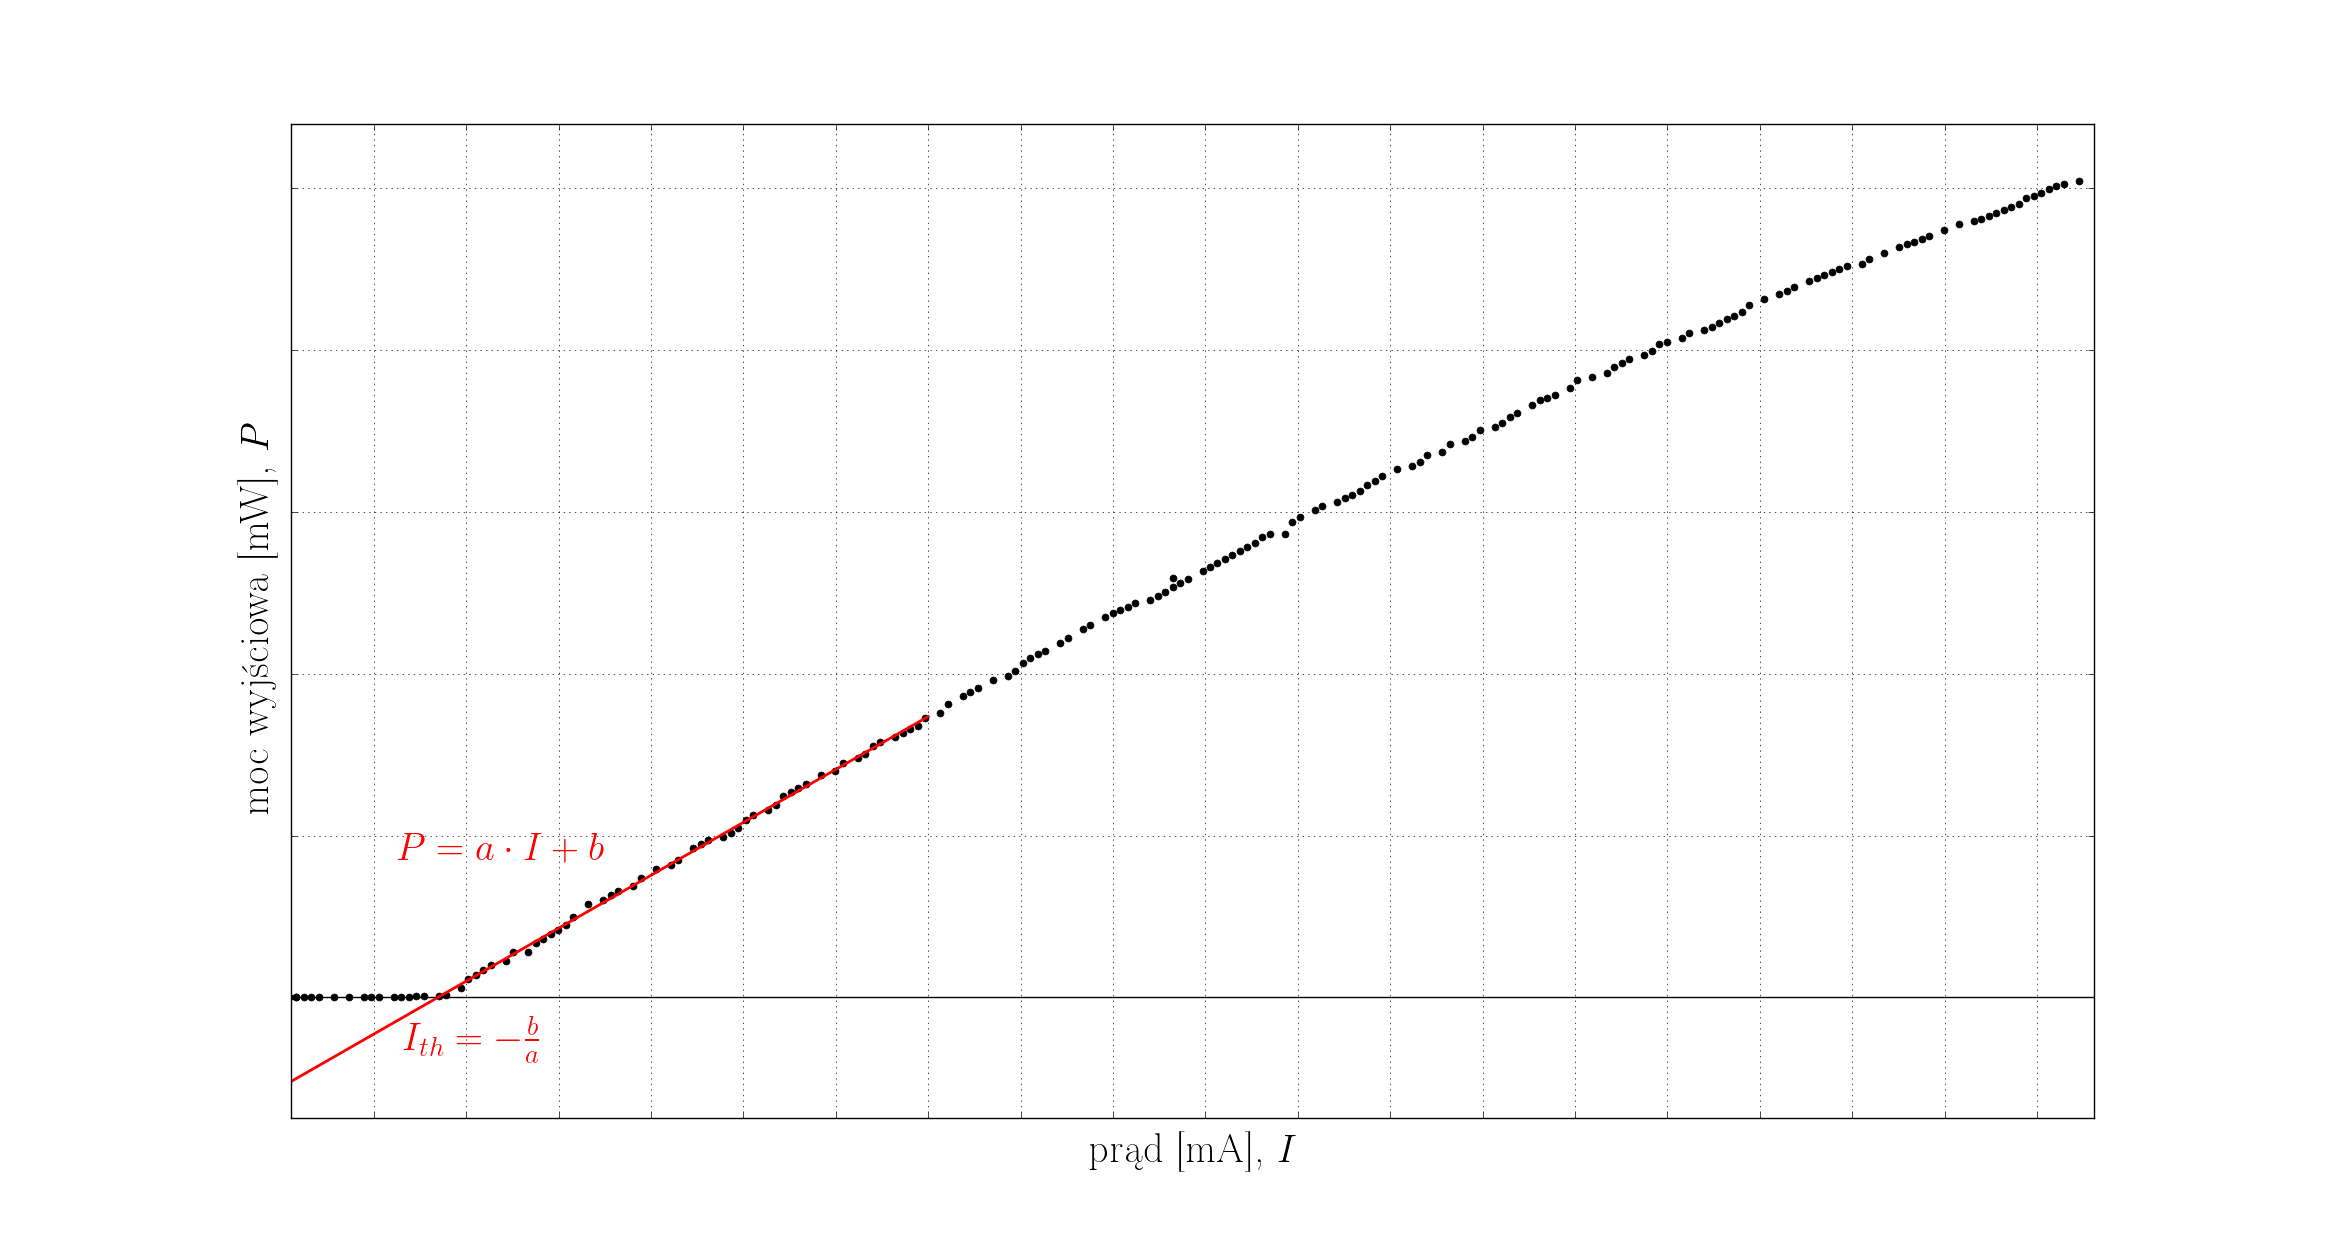
\includegraphics[scale=0.30]{plot_theory_i_th.png}
  \label{rys1}
  \caption{Charakterystyki wyjściowe lasera krawędziowego 980\,nm w różnych temperaturach. } 
\end{figure}
\newpage
Dla laserów krawędziowych zależności prądu progowego $I_{th}$ od temperatury $T$ możemy wyrazić za pomocą równania:
\begin{equation}
I_{th} = I_0 \exp \left( \frac{T}{T_0} \right)
\end{equation}
Wartości parametrów $I_0$ oraz $T_0$ możemy wyznaczyć na podstawie charakterystyk
emisyjnych lasera w różnych temperaturach $T$. \\
Przez zlogarytmowanie wartości prądu oraz podstawienie otrzymujemy:
\begin{equation}
\ln(I_{th}) =    \frac{T}{T_0}  + \ln(I_0)
\end{equation}
Mając wartości prądu progowego w danej temperaturze  można do nich dopasować funkcje liniową w postaci:
\begin{equation}
y = a \cdot T + b
\end{equation}
Gdzie:
\begin{equation}
y = \ln(I_{th})
\end{equation}
\begin{equation}
a = \frac{1}{T_0}
\end{equation}
\begin{equation}
b = \ln(I_0)
\end{equation}
Na tej podstawie możemy znaleźć poszukiwane parametry $I_0$ oraz $T_0$:
\begin{equation}
I_0 = \mathtt{e}^b
\end{equation}
\begin{equation}
T_0 = \frac{1}{a}
\end{equation}
Korzystając z różniczki zupełnej można obliczyć wartości błędów wyznaczonych wartości:
\begin{equation}
\Delta I_0 = \left\lvert \frac{\partial I_{0}}{\partial b} \right\rvert \cdot \Delta b = | b \mathtt{e}^b | \cdot \Delta b
\end{equation}
\begin{equation}
\Delta T_0 = \left\lvert \frac{\partial T_{0}}{\partial a} \right\rvert \cdot \Delta a = \left\lvert -\frac{1}{a^2} \right\rvert \cdot \Delta a
\end{equation}
\subsection{Sprawność}
Innym ważnym parametrem, którym możemy scharakteryzować lasery półprzewodnikowe jest ich sprawność. Można wyróżnić następujące sprawności:
\begin{itemize}
\item Sprawność różniczkowa (ang. \textit{slope efficiency}) --- jest zdefiniowana jako nachylenie krzywej uzyskanej przez wykreślenie zależności mocy wyjściowej z lasera versus energii dostarczonej do lasera (natężenie prądu lub moc dostarczona).
\item Sprawność całkowita (ang. \textit{Wall-plug-efficiency}) --- jest zdefiniowana jako stosunek mocy wyjściowej do całkowitej mocy wejściowej lasera.
\end{itemize}
%
\newpage








\section{Badanie lasera}
\subsection{Laser 980\,nm}
Podpunkt ten zawiera wyniki pomiarów dla lasera krawędziowego o emitowanej fali długości 980\,nm.
Pomiar polegał w pierwszej części na wykonaniu charakterystyk prądowo-napięciowych
oraz prądowo-oświetleniowych lasera w temperaturze lasera od 283\,K do 363\,K krokiem co 10\,K.
Na podstawie otrzymanych charakterystyk wyznaczyłem wartość prądu progowego w danej temperaturze.
Następnie korzystając z wyznaczonych wartość na podstawie wzorów~(5.7) i (5.8) znalazłem
parametry $I_{0} = (89.9 \pm 0.1)$\,mA oraz $T_0 = (0.04 \pm 0.01)$\,K.

Tabela 1 zawiera wyznazone wartości prądu progowego $I_0$ dla tego lasera. Rysunek 5.1 przedstawia charakterystykę wszystkich badanych laserów. Rysunki 5.2-5.29 przedstawiają charakterystyki lasera wraz z oblicoznymi paramenrami które słuzą do charakterystyki lasera. Rysunek 5.13 przedstawia wykres prądu progowego w funkcji temperatury. \\ 

\begin{table}[h!]
\begin{center}
\caption{ Wyznaczone wartośc prądu progowego $I_0$ w różnych temperaturach $T$ dla lasera krawędziowego 980\,nm. }
\begin{tabular}{ | C{3.5cm}|  C{3.5cm} | C{3.5cm} | C{3.5cm}|}
\hline
$T$ [K] &   $I_{th}$ [mA]   \\ \hline
283      &   1.0 $\pm$ 0.1  \\ \hline
293      &   1.0 $\pm$ 0.1  \\ \hline
303      &   1.1 $\pm$ 0.1  \\ \hline
313      &   1.2 $\pm$ 0.1  \\ \hline
323      &   1.3 $\pm$ 0.1  \\ \hline
333      &   1.5 $\pm$ 0.1  \\ \hline
343      &   1.7 $\pm$ 0.1  \\ \hline
353      &   2.0 $\pm$ 0.1  \\ \hline
363      &   2.4 $\pm$ 0.1  \\ \hline
\end{tabular}
\end{center}
\end{table}

\newpage


\begin{figure}
\center
  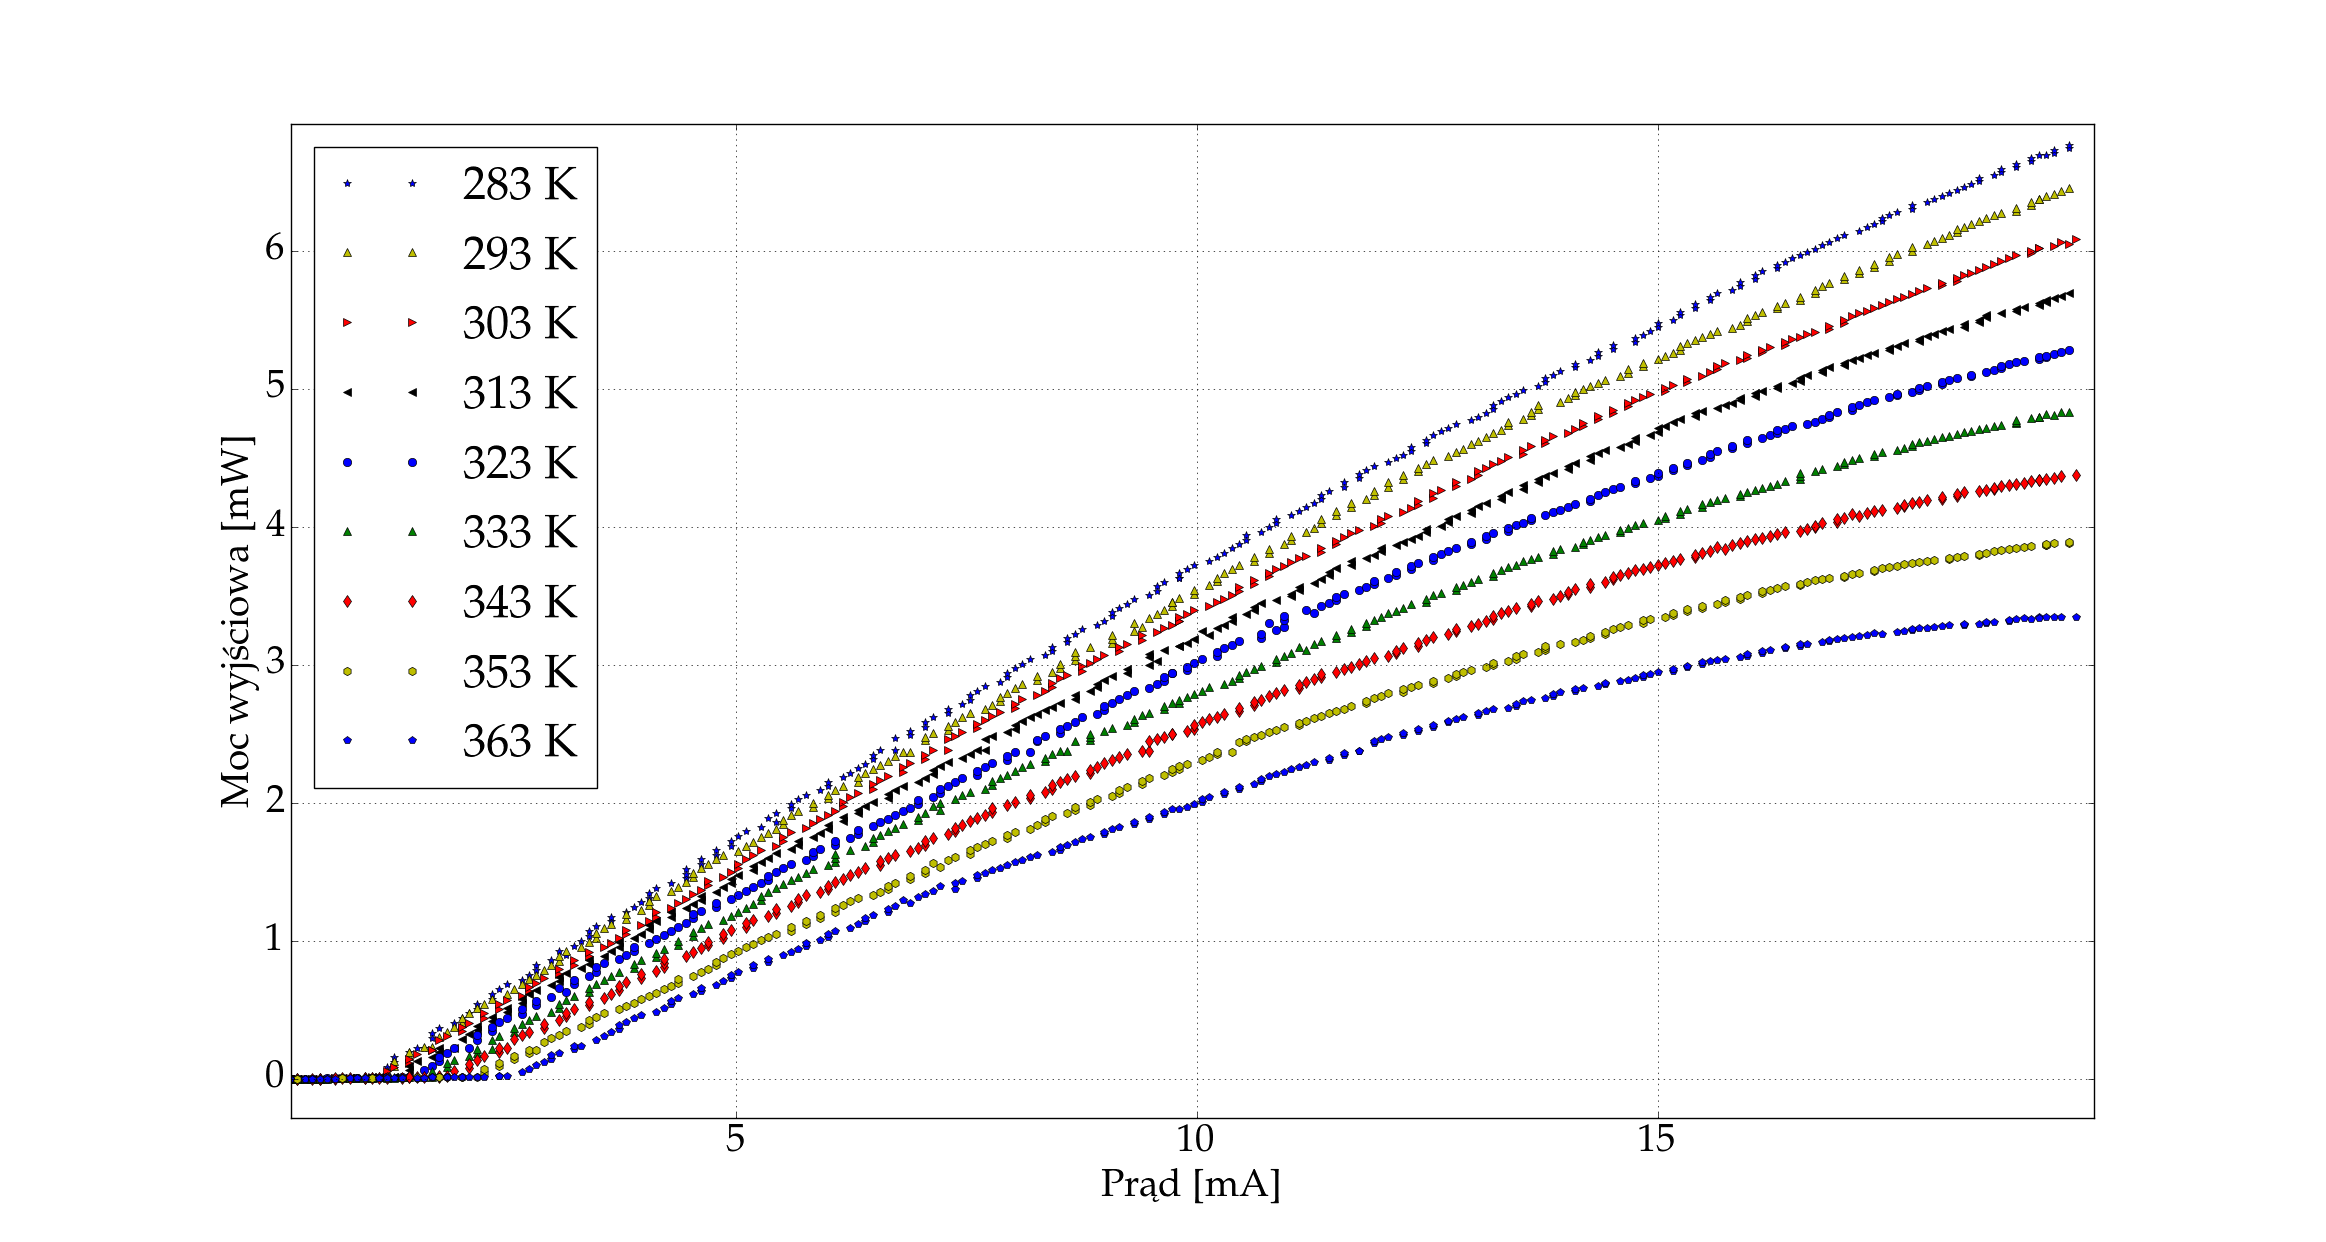
\includegraphics[scale=0.30]{plot980/plot_all.png}
  \label{rys1}
  \caption{Charakterystyki wyjściowe lasera krawędziowego 980\,nm w różnych temperaturach. } 
\end{figure}

\subsection{Laser VCSEL 850\,nm}
Laser 850
\begin{table}[h!]
\begin{center}
\caption{ Wyznaczone wartośc prądu progowego $I_0$ w różnych temperaturach $T$ dla lasera VCSEL 850\,nm. }
\begin{tabular}{ | C{3.5cm}|  C{3.5cm} | C{3.5cm} | C{3.5cm}|}
\hline
$T$ [K] &   $I_{th}$ [mA]   \\ \hline
283      &   1.70 $\pm$ 0.03  \\ \hline
288      &   1.67 $\pm$ 0.03  \\ \hline
293		 &   1.60 $\pm$ 0.03  \\ \hline
298		 &   1.55 $\pm$ 0.04  \\ \hline 
303		 &   1.59 $\pm$ 0.03  \\ \hline
308		 &   1.63 $\pm$ 0.03  \\ \hline
313		 &   1.65 $\pm$ 0.03  \\ \hline
318		 &   1.68 $\pm$ 0.04  \\ \hline      
323		 &   1.73 $\pm$ 0.04  \\ \hline
328		 &   1.83 $\pm$ 0.04  \\ \hline
333		 &   1.89 $\pm$ 0.04  \\ \hline
338		 &   2.01 $\pm$ 0.04  \\ \hline
343		 &   2.14 $\pm$ 0.04  \\ \hline
348		 &   2.24 $\pm$ 0.05  \\ \hline
353		 &   2.38 $\pm$ 0.05  \\ \hline
358		 &   2.57 $\pm$ 0.05  \\ \hline
363		 &   2.74 $\pm$ 0.07  \\ \hline         
\end{tabular}
\end{center}
\end{table}
\begin{figure}
\center
  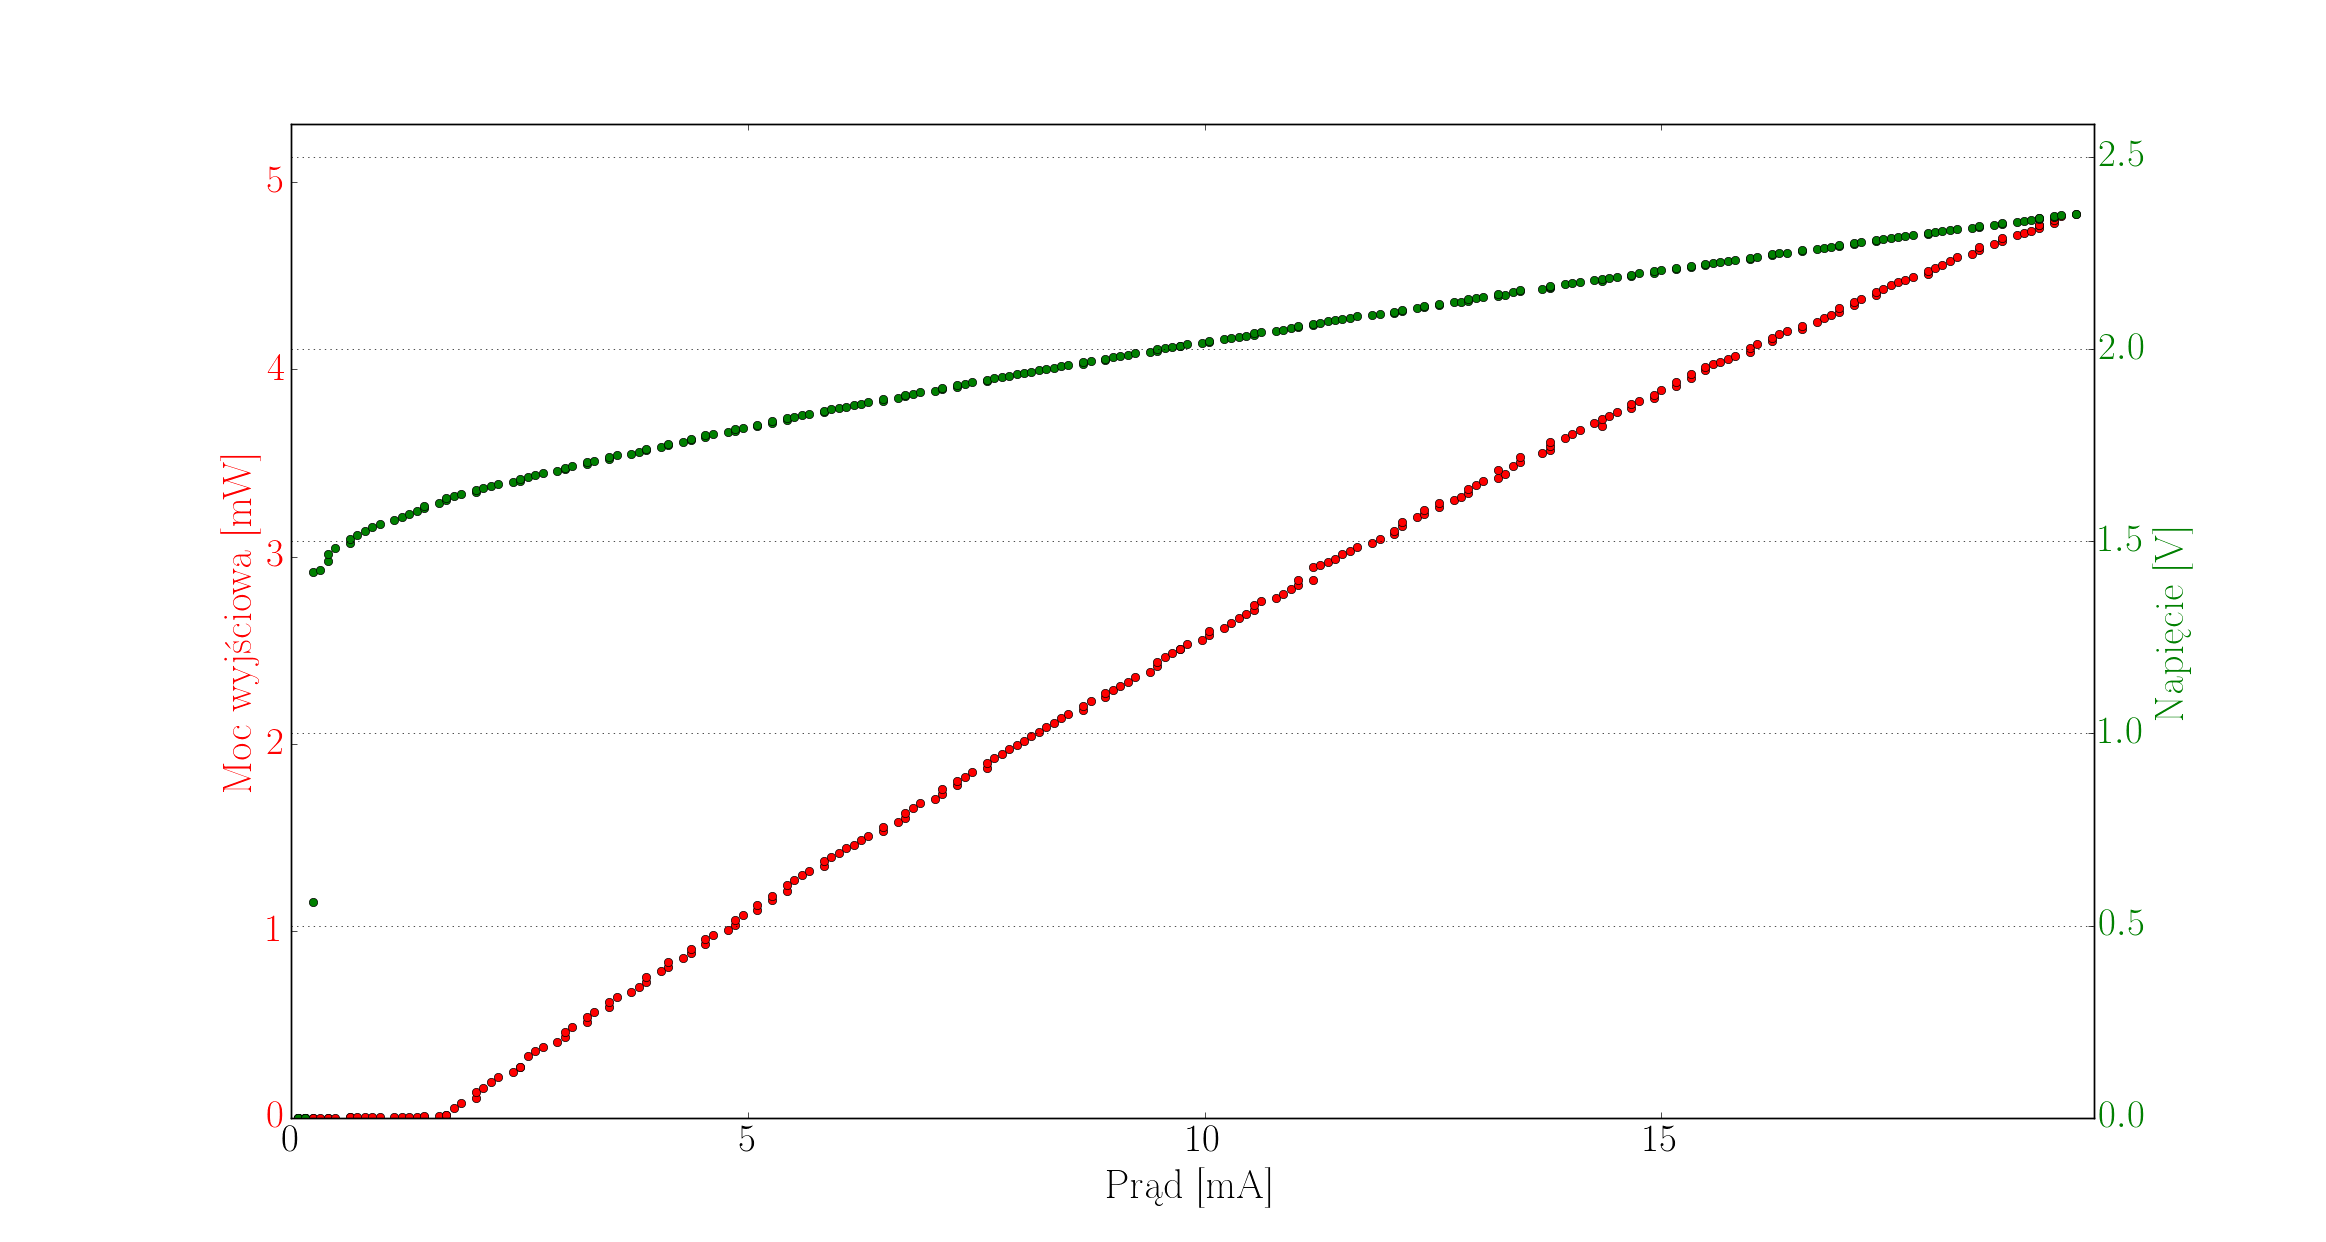
\includegraphics[scale=0.30]{plot_vcsel850/temp_20_ivl.png}
  \label{rys1}
  \caption{Charakterystyki wyjściowe lasera VCSEL 850\,nm w temperaturze 293 K. } 
\end{figure}
\begin{figure}
\center
  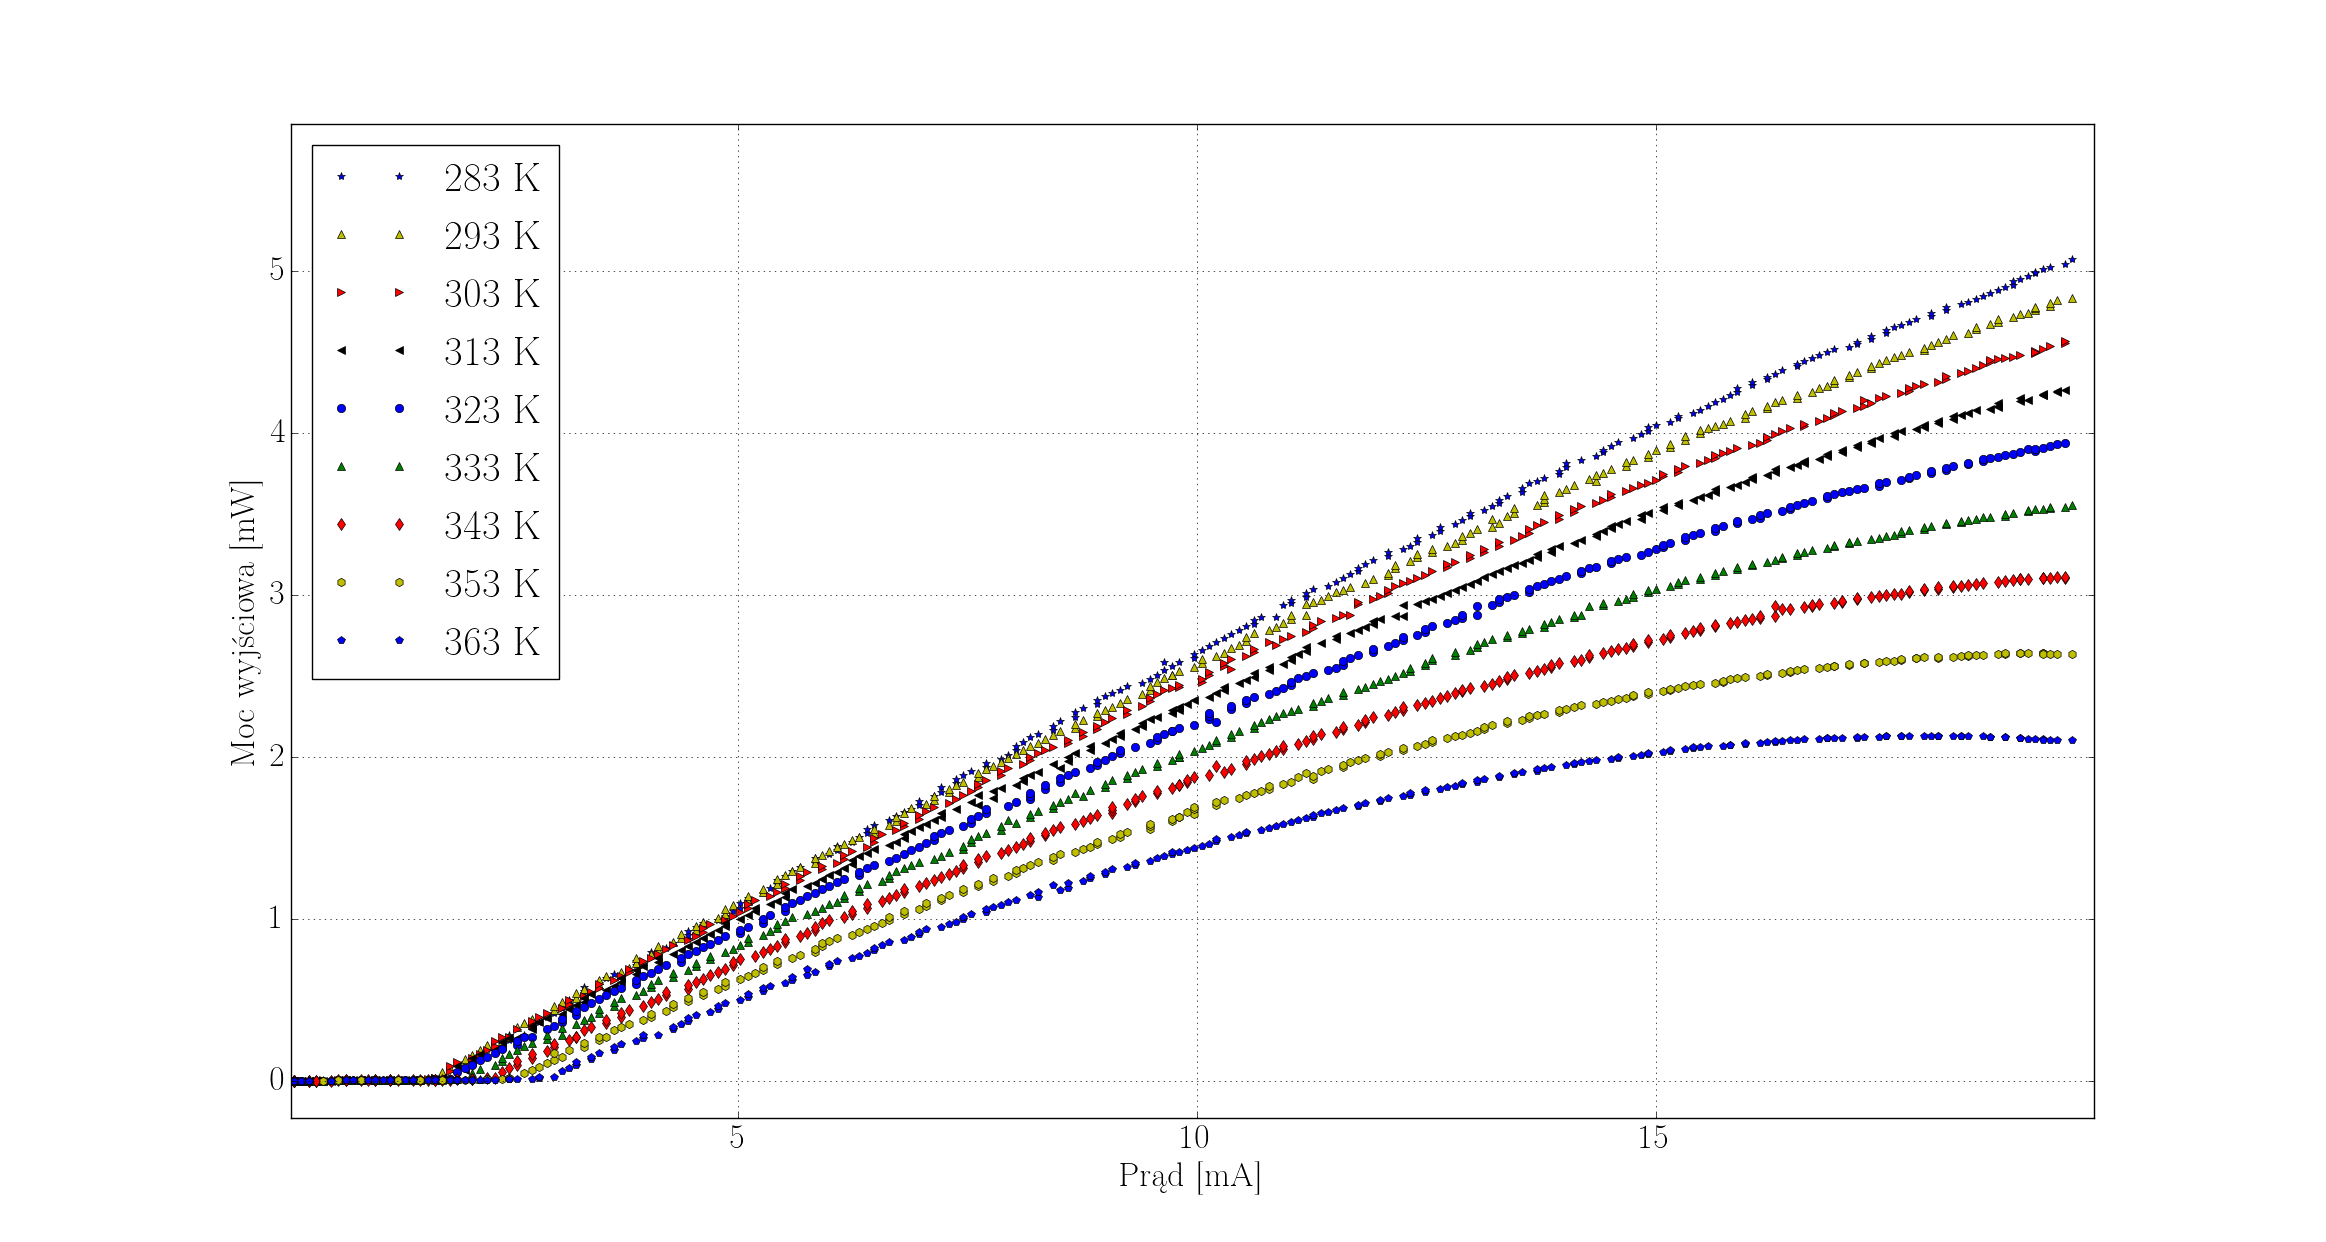
\includegraphics[scale=0.30]{plot_vcsel850/plot_all.png}
  \label{rys1}
  \caption{Charakterystyki wyjściowe lasera VCSEL 850\,nm w różnych temperaturach.} 
\end{figure}
\begin{figure}
\center
  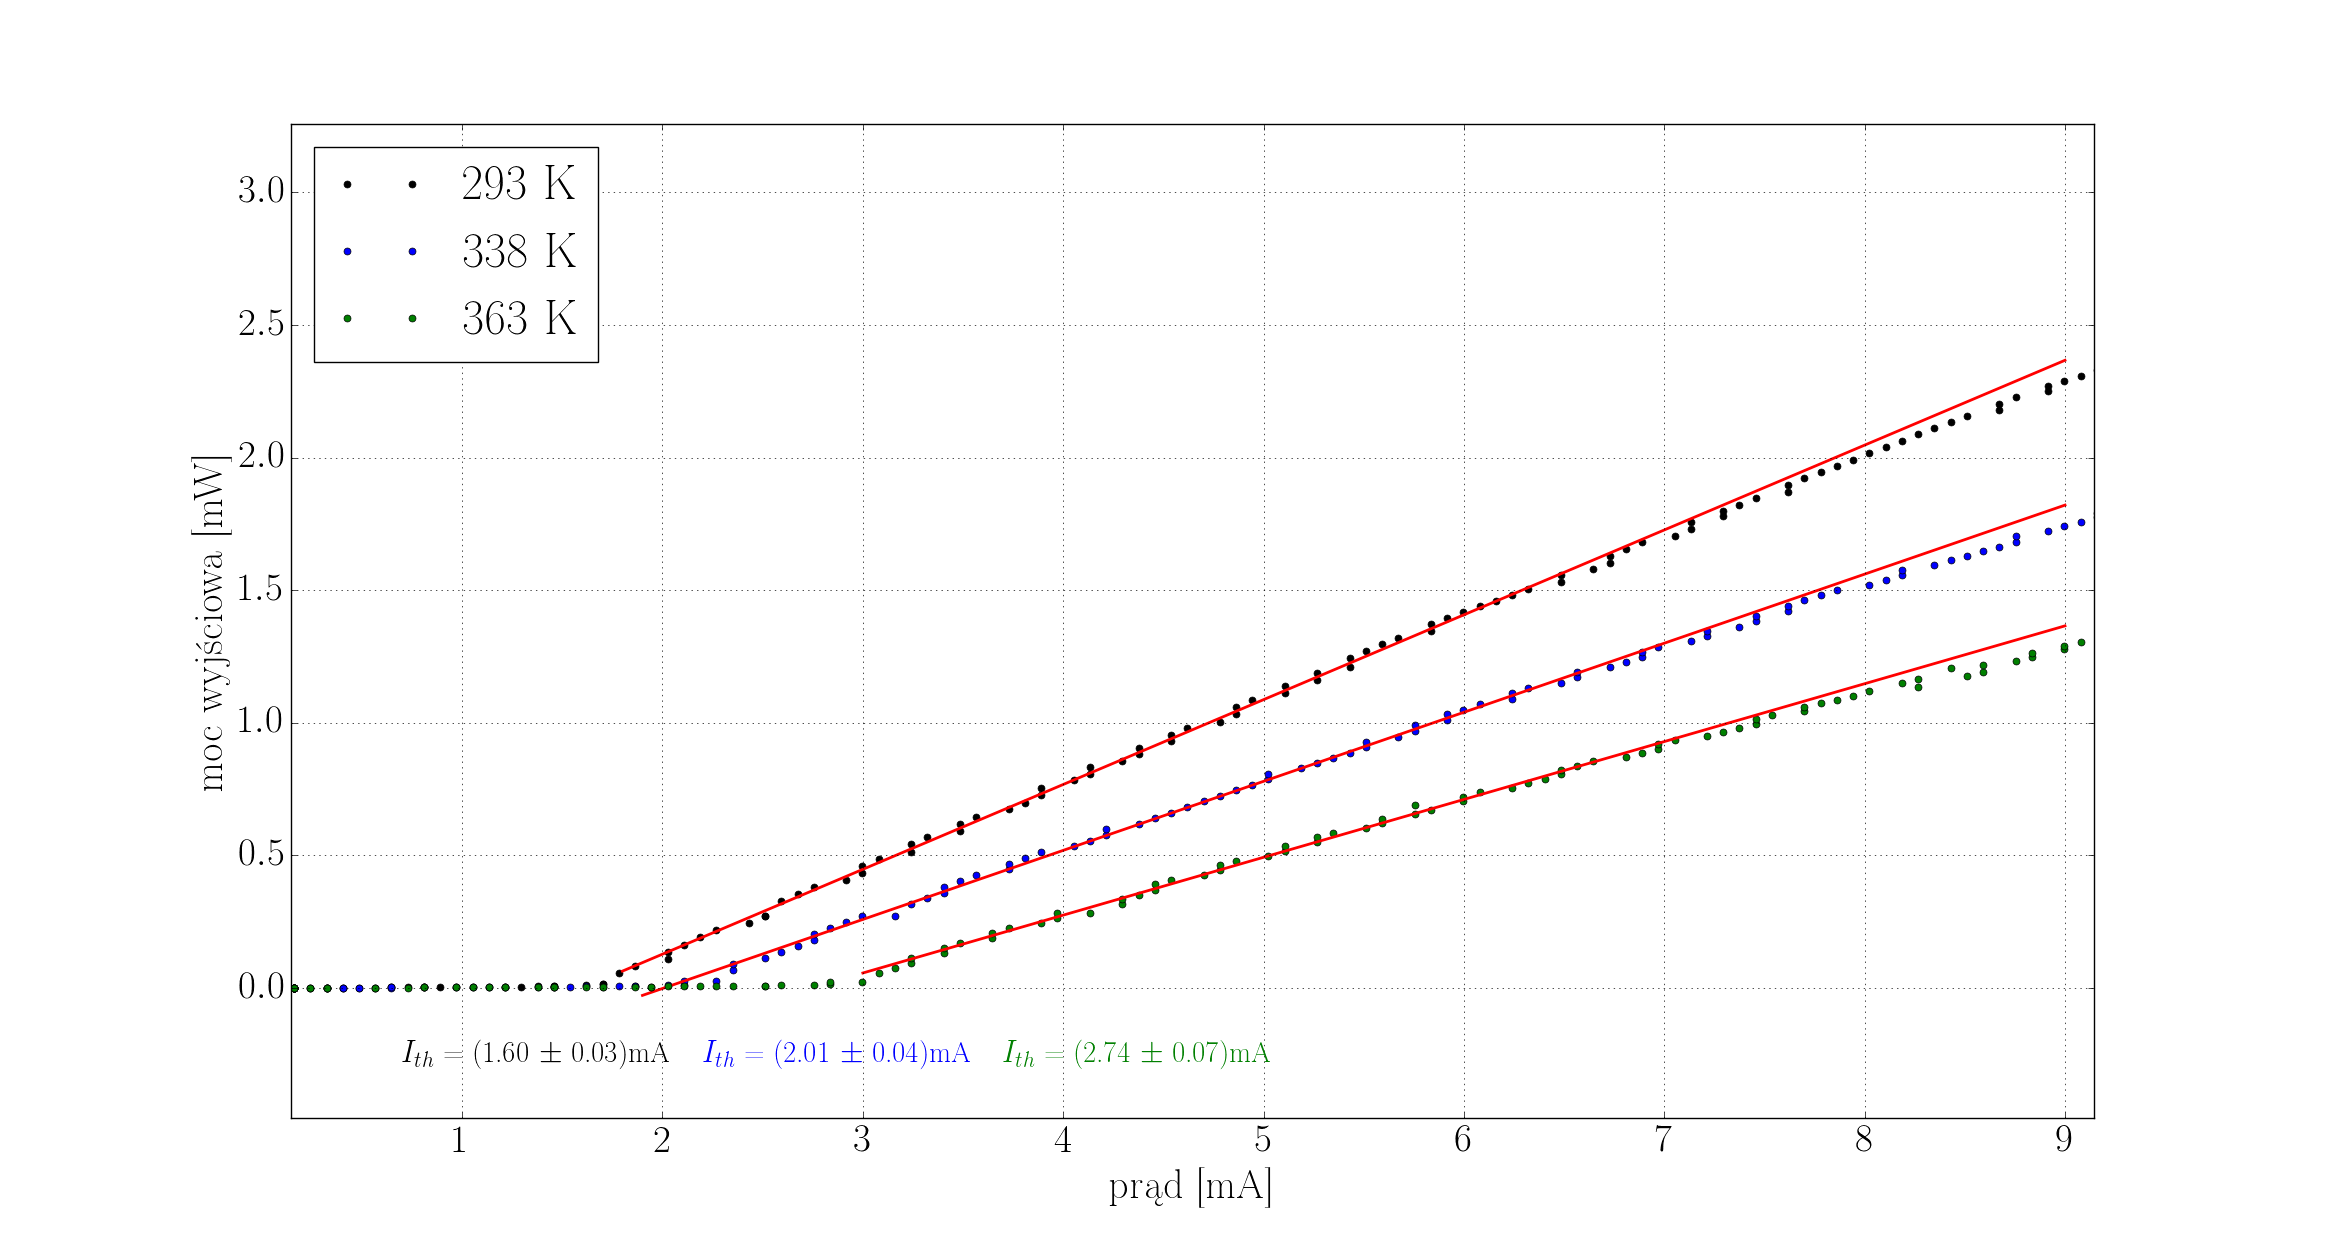
\includegraphics[scale=0.30]{plot_vcsel850/plot_3_i_th.png}
  \label{rys1}
  \caption{Charakterystyki wyjściowe lasera VCSEL 850\,nm z wyznaczonym prądem progowym $I_{th}$ w różnych temperaturach.} 
\end{figure}
\begin{figure}
\center
  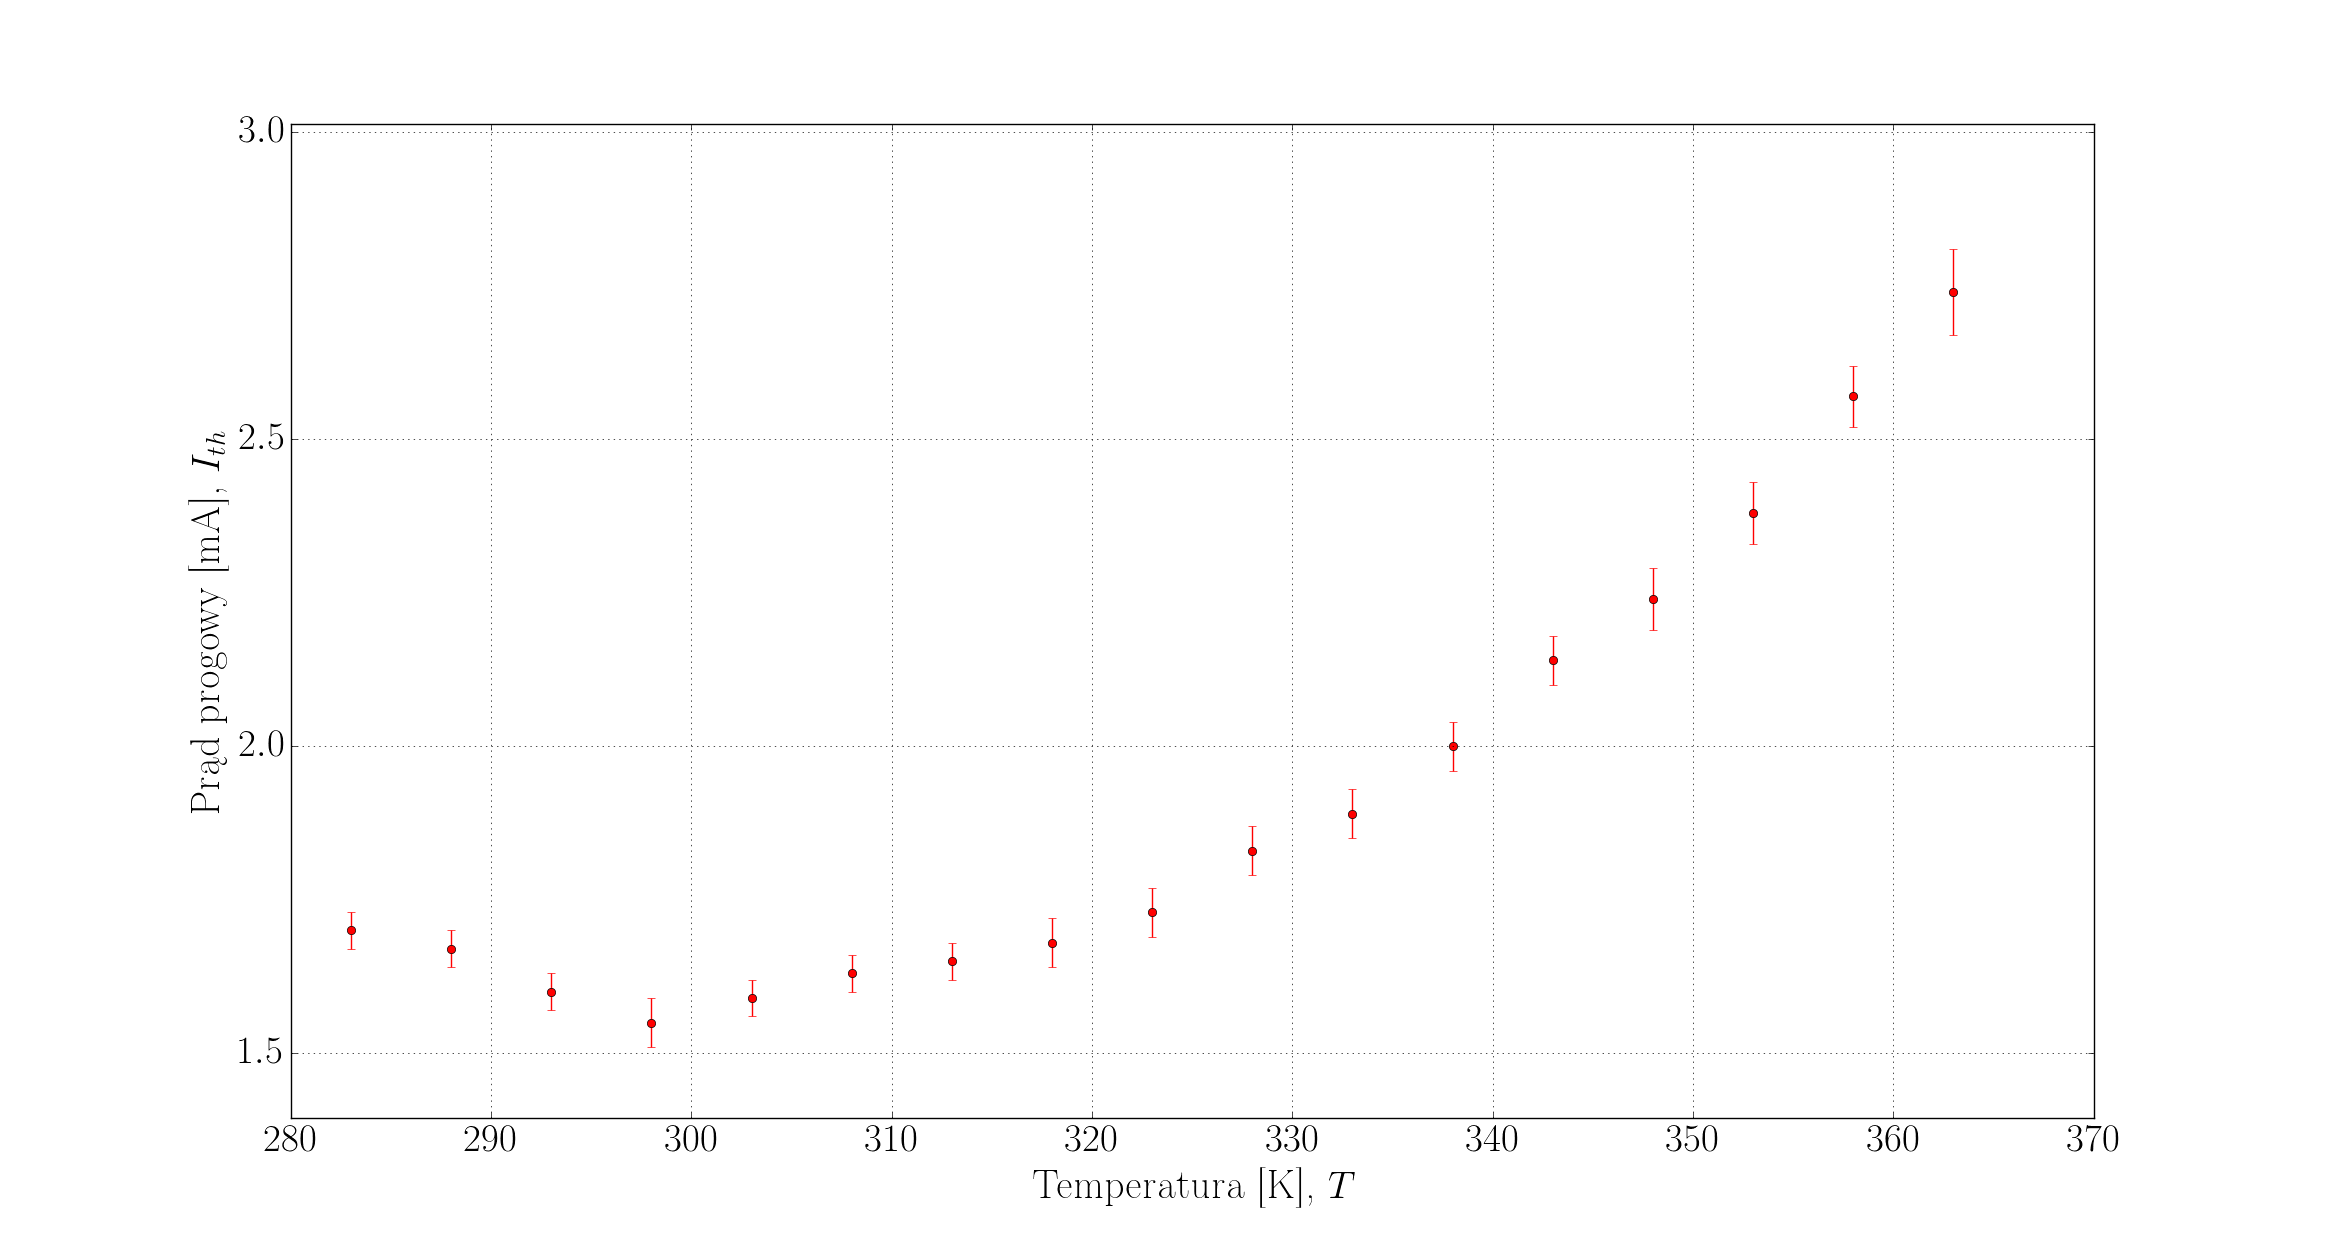
\includegraphics[scale=0.30]{plot_vcsel850/plot_lin_i_th.png}
  \label{rys1}
  \caption{Wykres prądu progowego w zależności od temperatury dla lasera VCSEL 850 \,nm.} 
\end{figure}
\begin{figure}
\center
  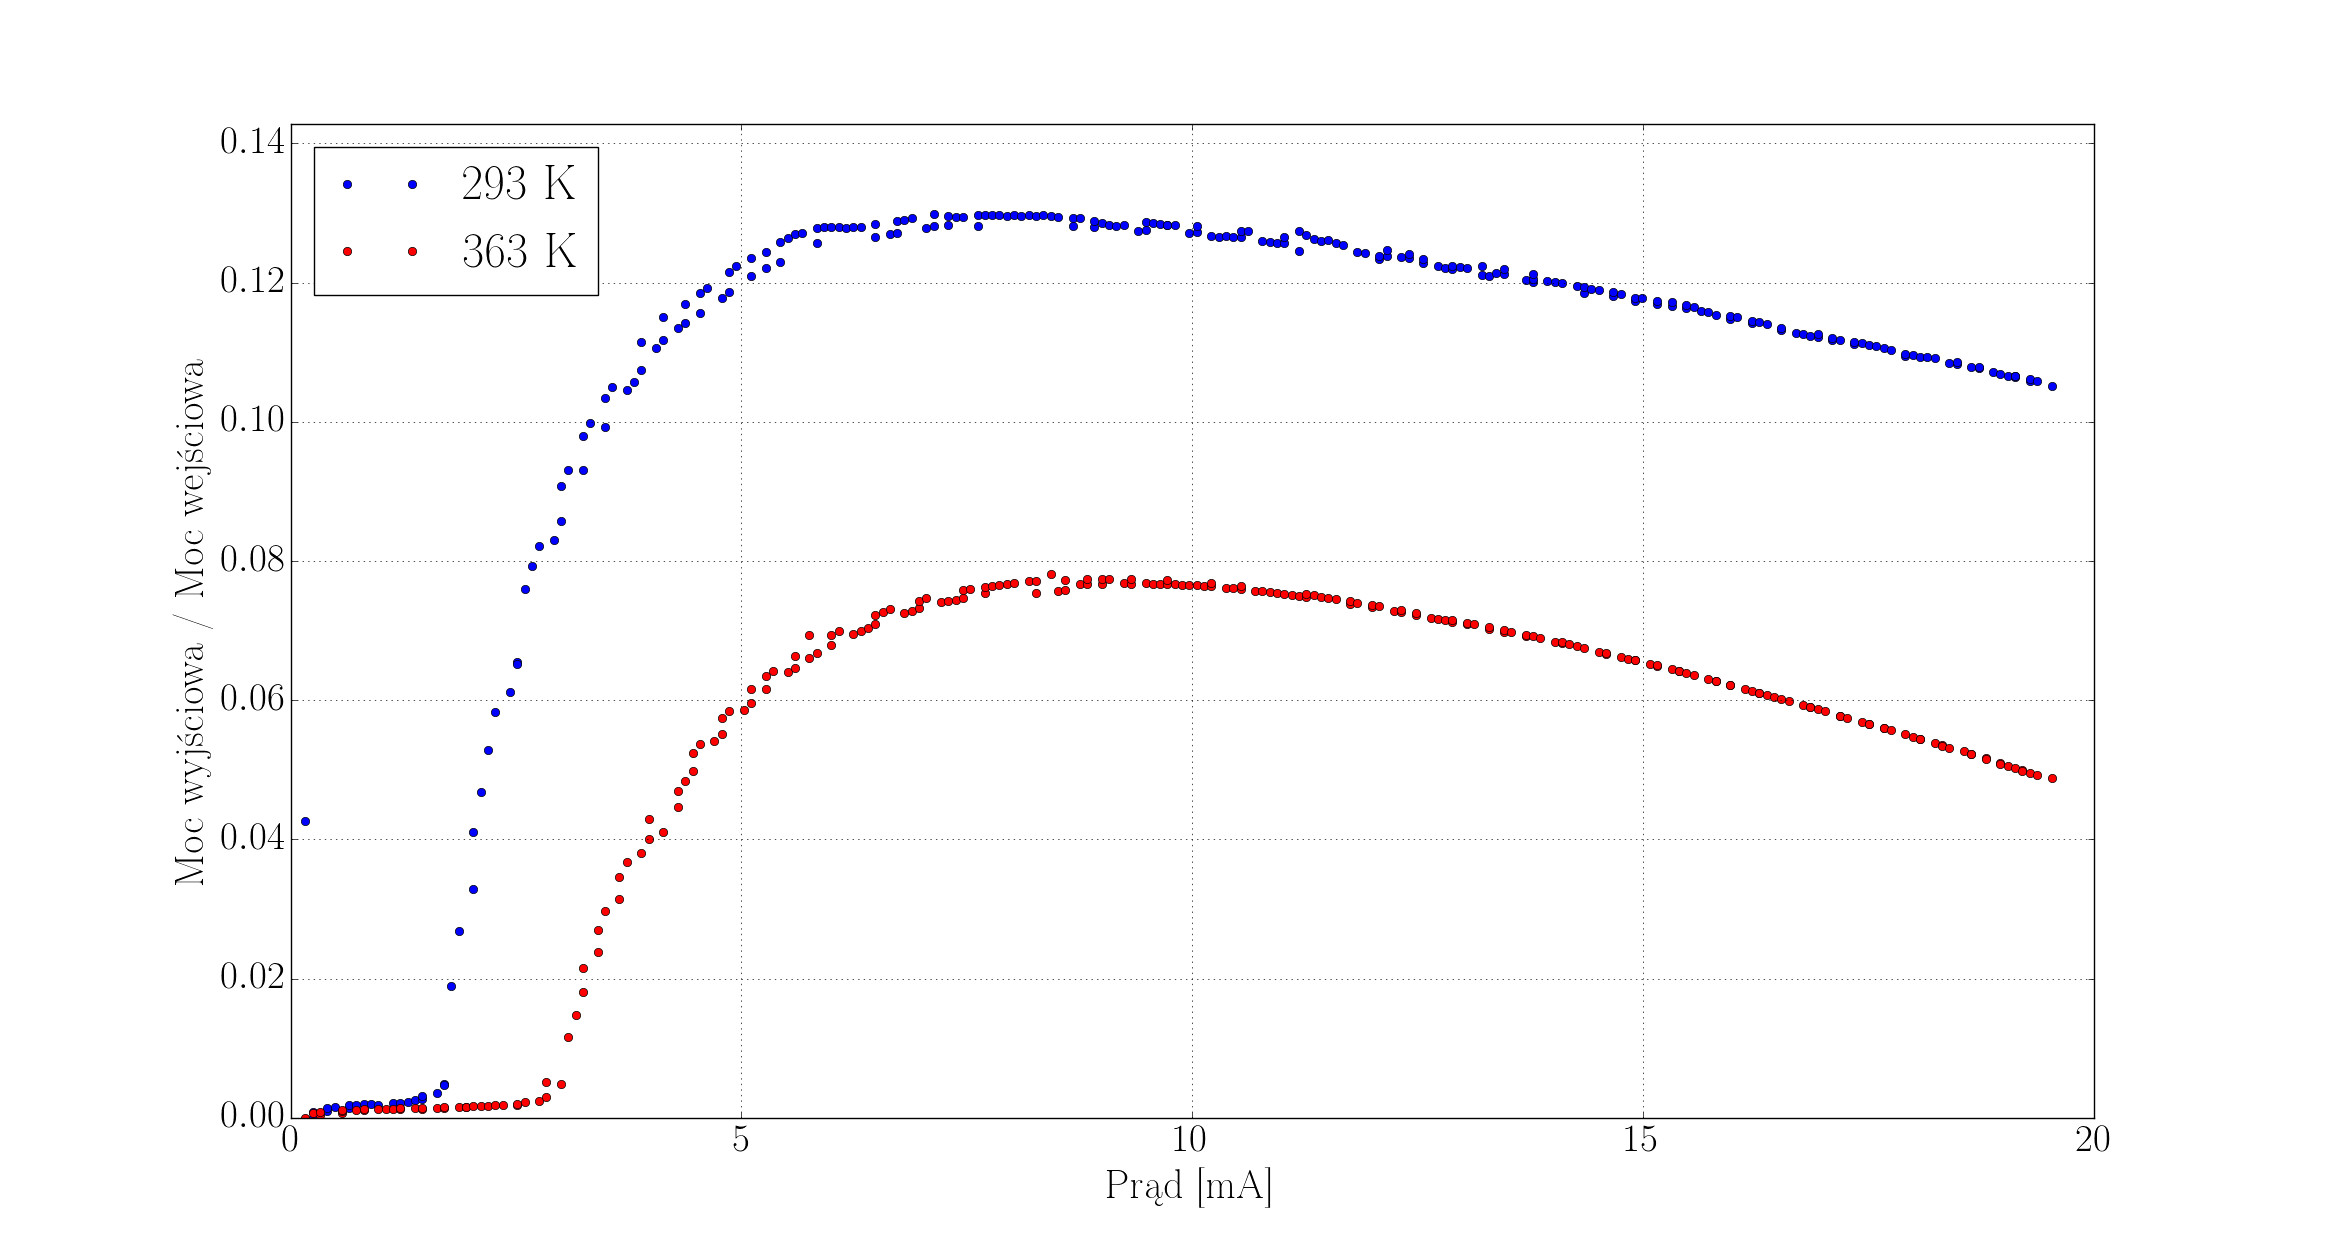
\includegraphics[scale=0.30]{plot_vcsel850/plot_eff.png}
  \label{rys1}
  \caption{Wykres sprawności lasera VCSEL 850\,nm.} 
\end{figure}
\begin{figure}
\center
  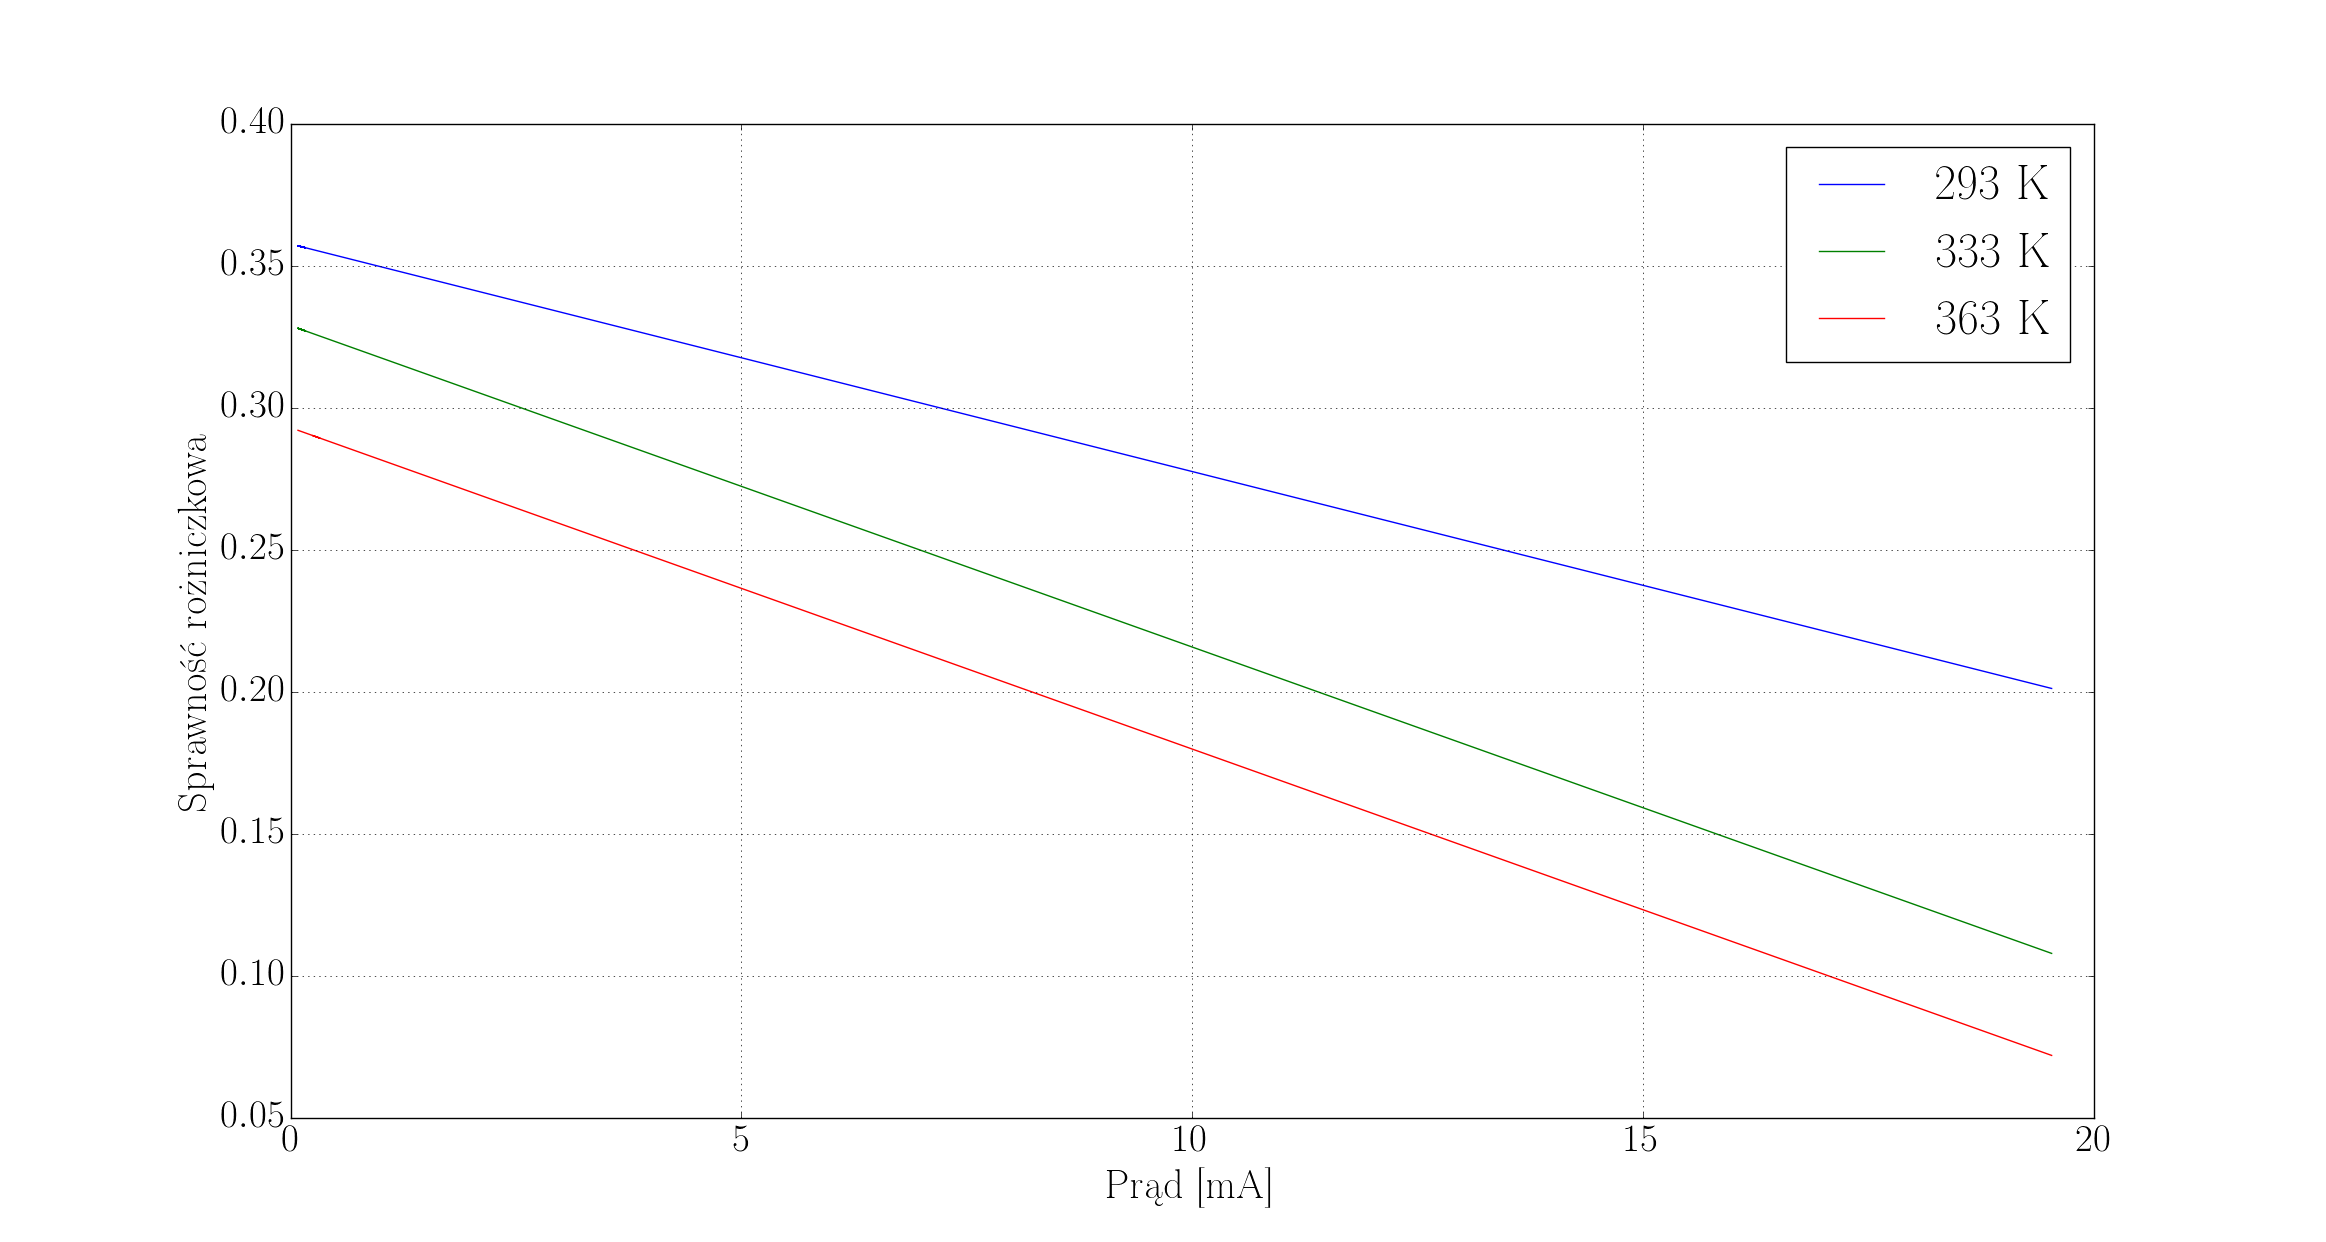
\includegraphics[scale=0.30]{plot_vcsel850/plot_slope_eff_via_current.png}
  \label{rys1}
  \caption{Wykres sprawności różniczkowej lasera VCSEL 850\,nm w funkcja prądu wejściowego.} 
\end{figure}
\begin{figure}
\center
  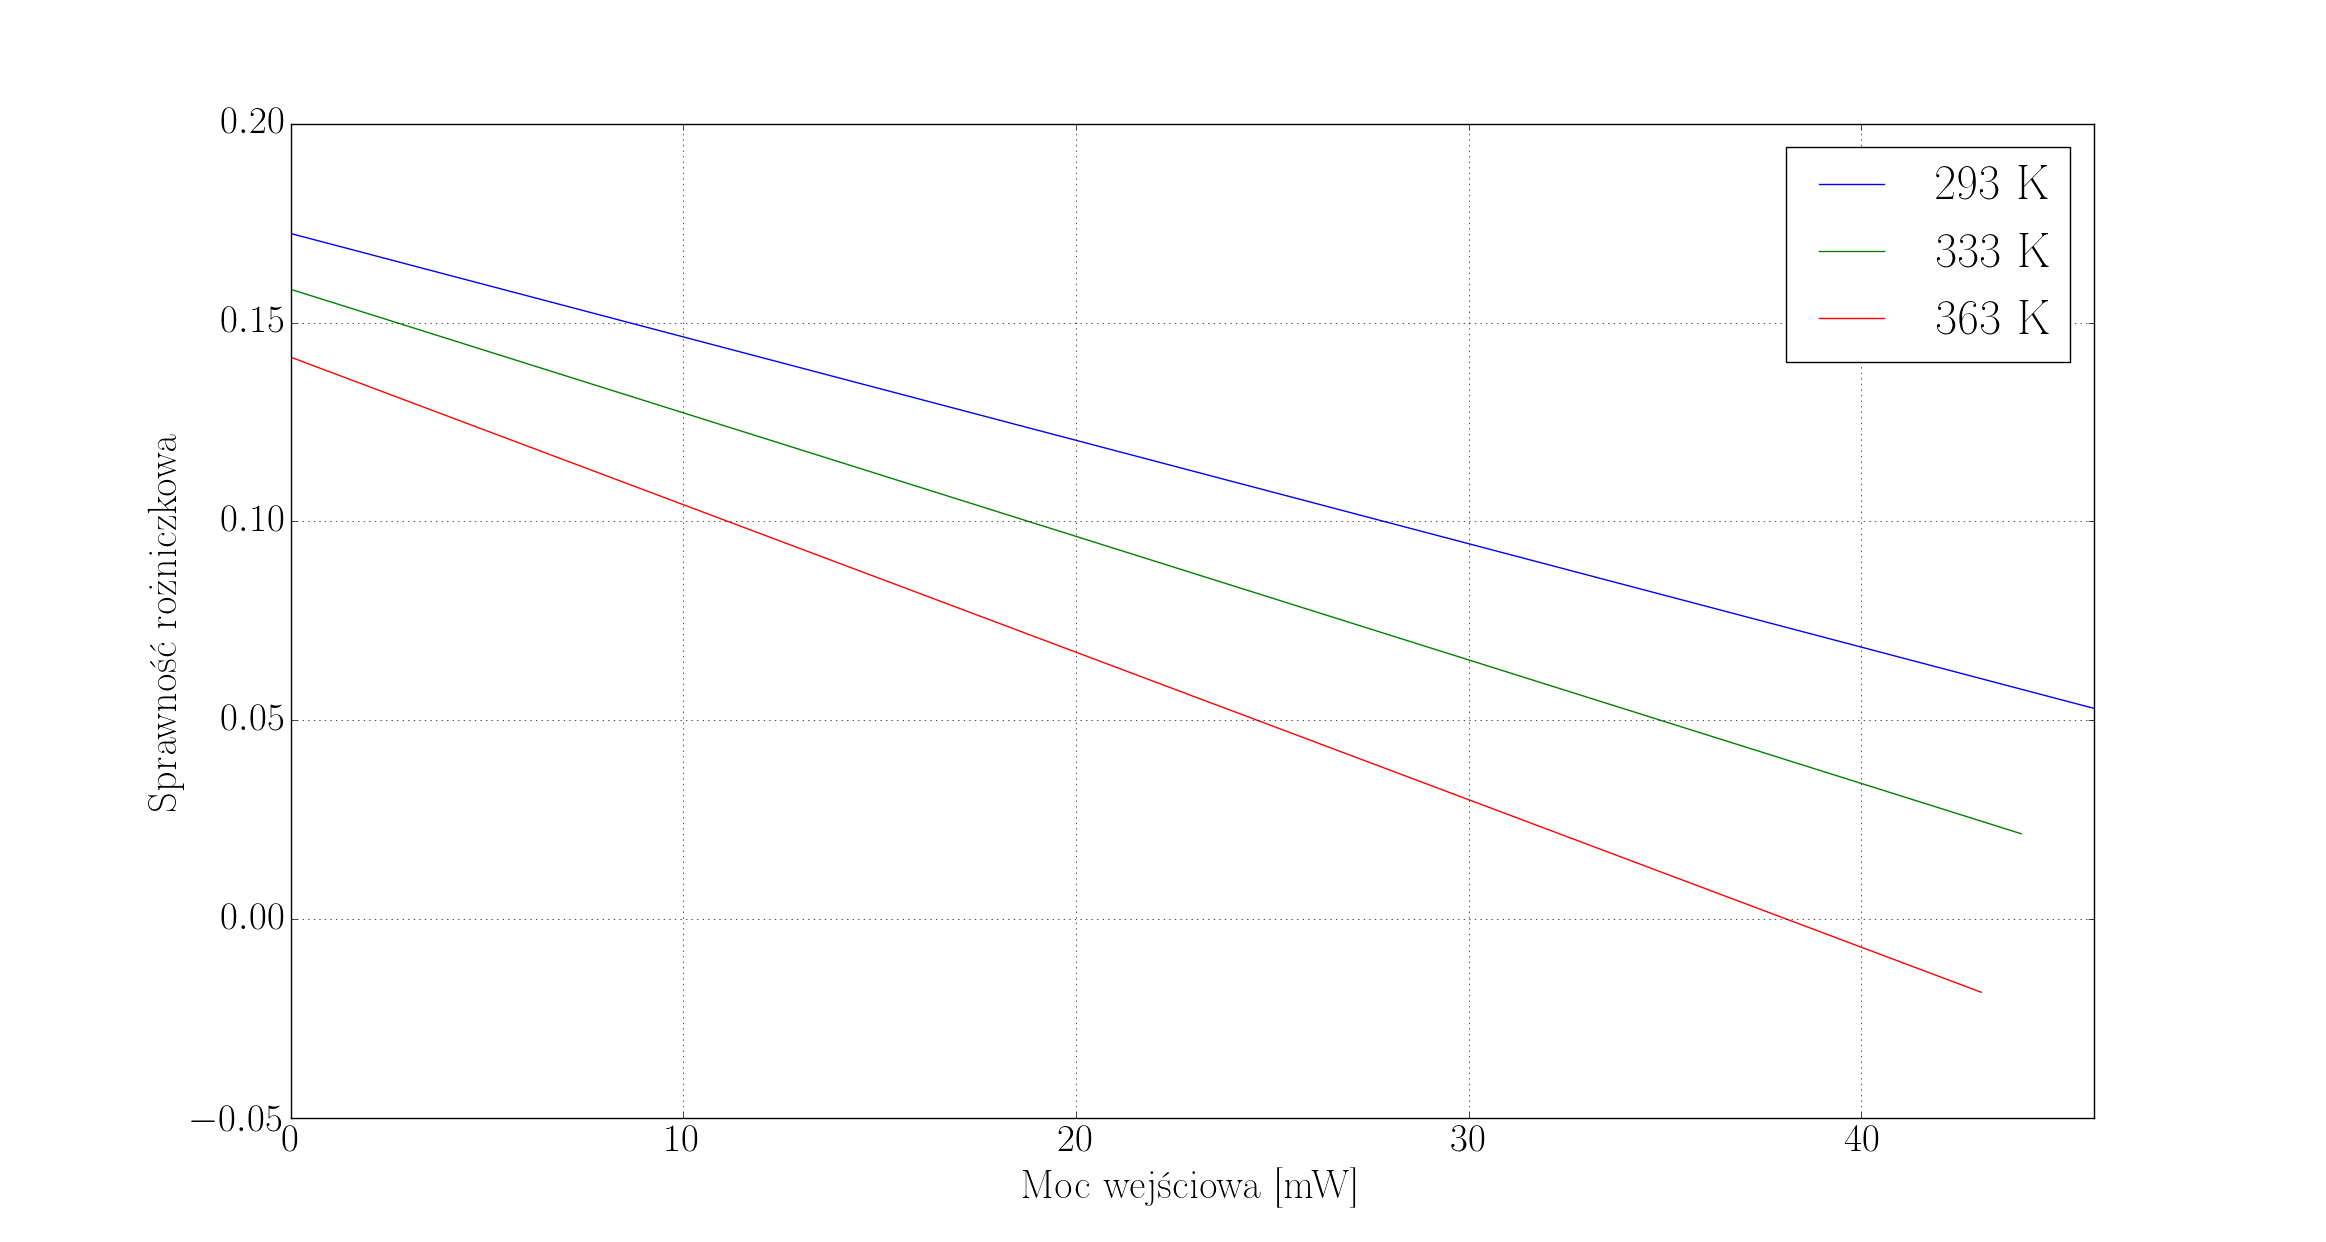
\includegraphics[scale=0.30]{plot_vcsel850/plot_slope_eff_via_power.png}
  \label{rys1}
  \caption{Wykres sprawności różniczkowej lasera VCSEL 850\,nm w funkcja mocy wejściowej.} 
\end{figure}
\subsection{Laser krawędziowy 635\,nm} 
\begin{table}
\begin{center}
\caption{ Wyznaczone wartośc prądu progowego $I_0$ w różnych temperaturach $T$ dla lasera krawędziowego 635\,nm. }
\begin{tabular}{ | C{3.5cm}|  C{3.5cm} | C{3.5cm} | C{3.5cm}|}
\hline
$T$ [K] &   $I_{th}$ [mA]   \\ \hline
293      &   22.4 $\pm$ 0.3  \\ \hline
298      &   25.0 $\pm$ 0.2  \\ \hline
303      &   28.1 $\pm$ 0.3  \\ \hline
308      &   31.3 $\pm$ 0.6  \\ \hline
313      &   35.7 $\pm$ 0.9  \\ \hline
\end{tabular}
\end{center}
\end{table}

\begin{figure}
\center
  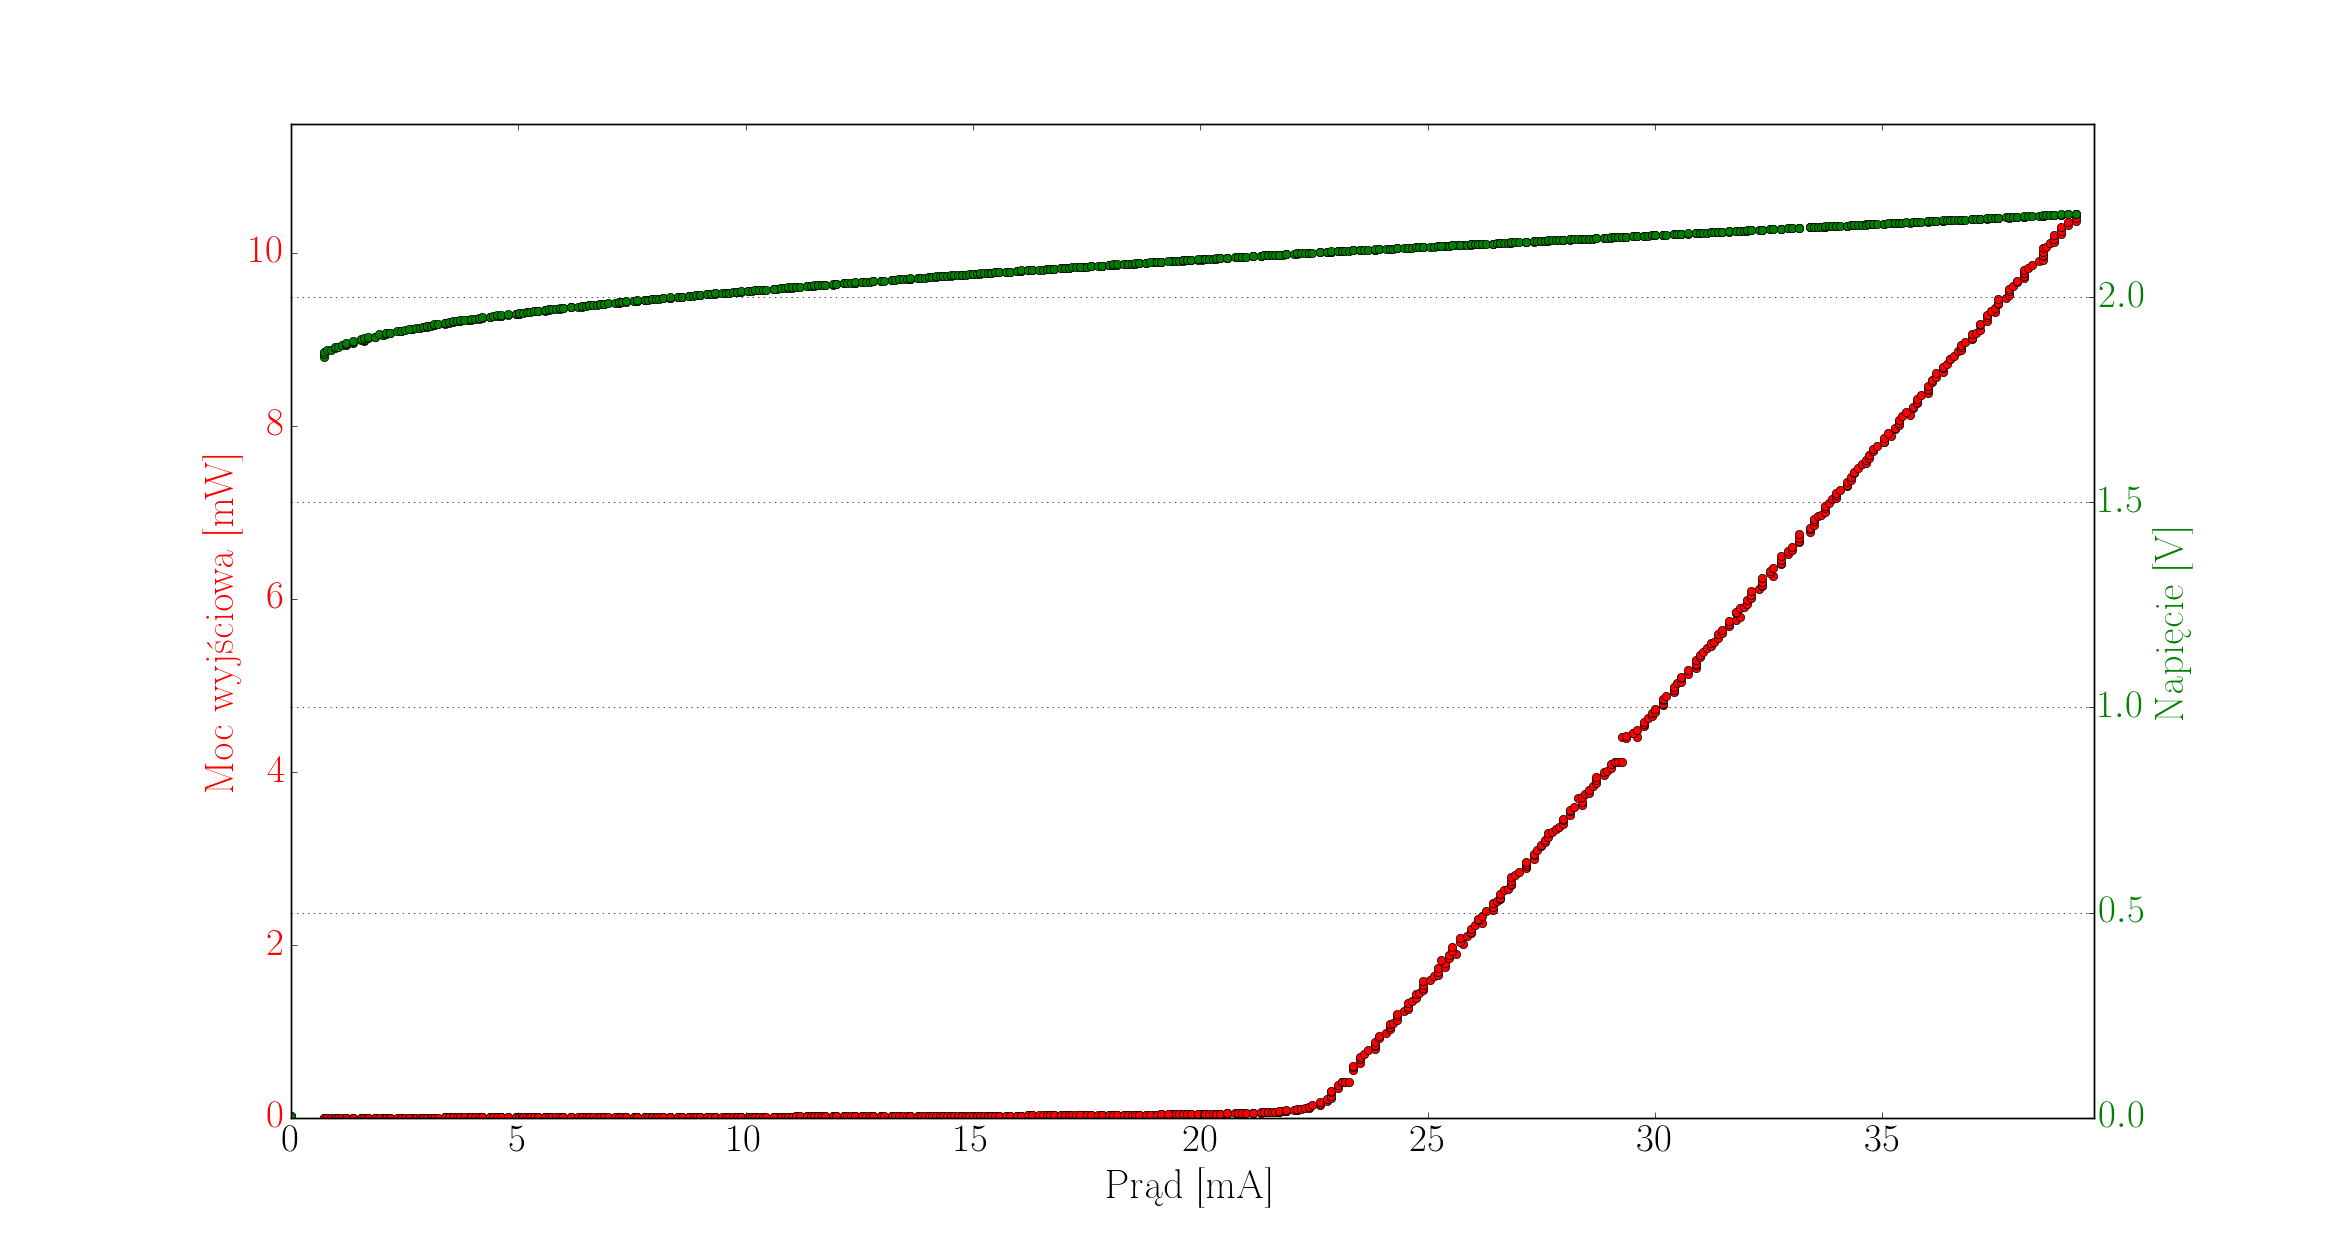
\includegraphics[scale=0.30]{plot635/plot_ivl_20.png}
  \label{rys1}
  \caption{Charakterystyka wyjściowa lasera krawędziowego 635 \,nm.} 
\end{figure}

\begin{figure}
\center
  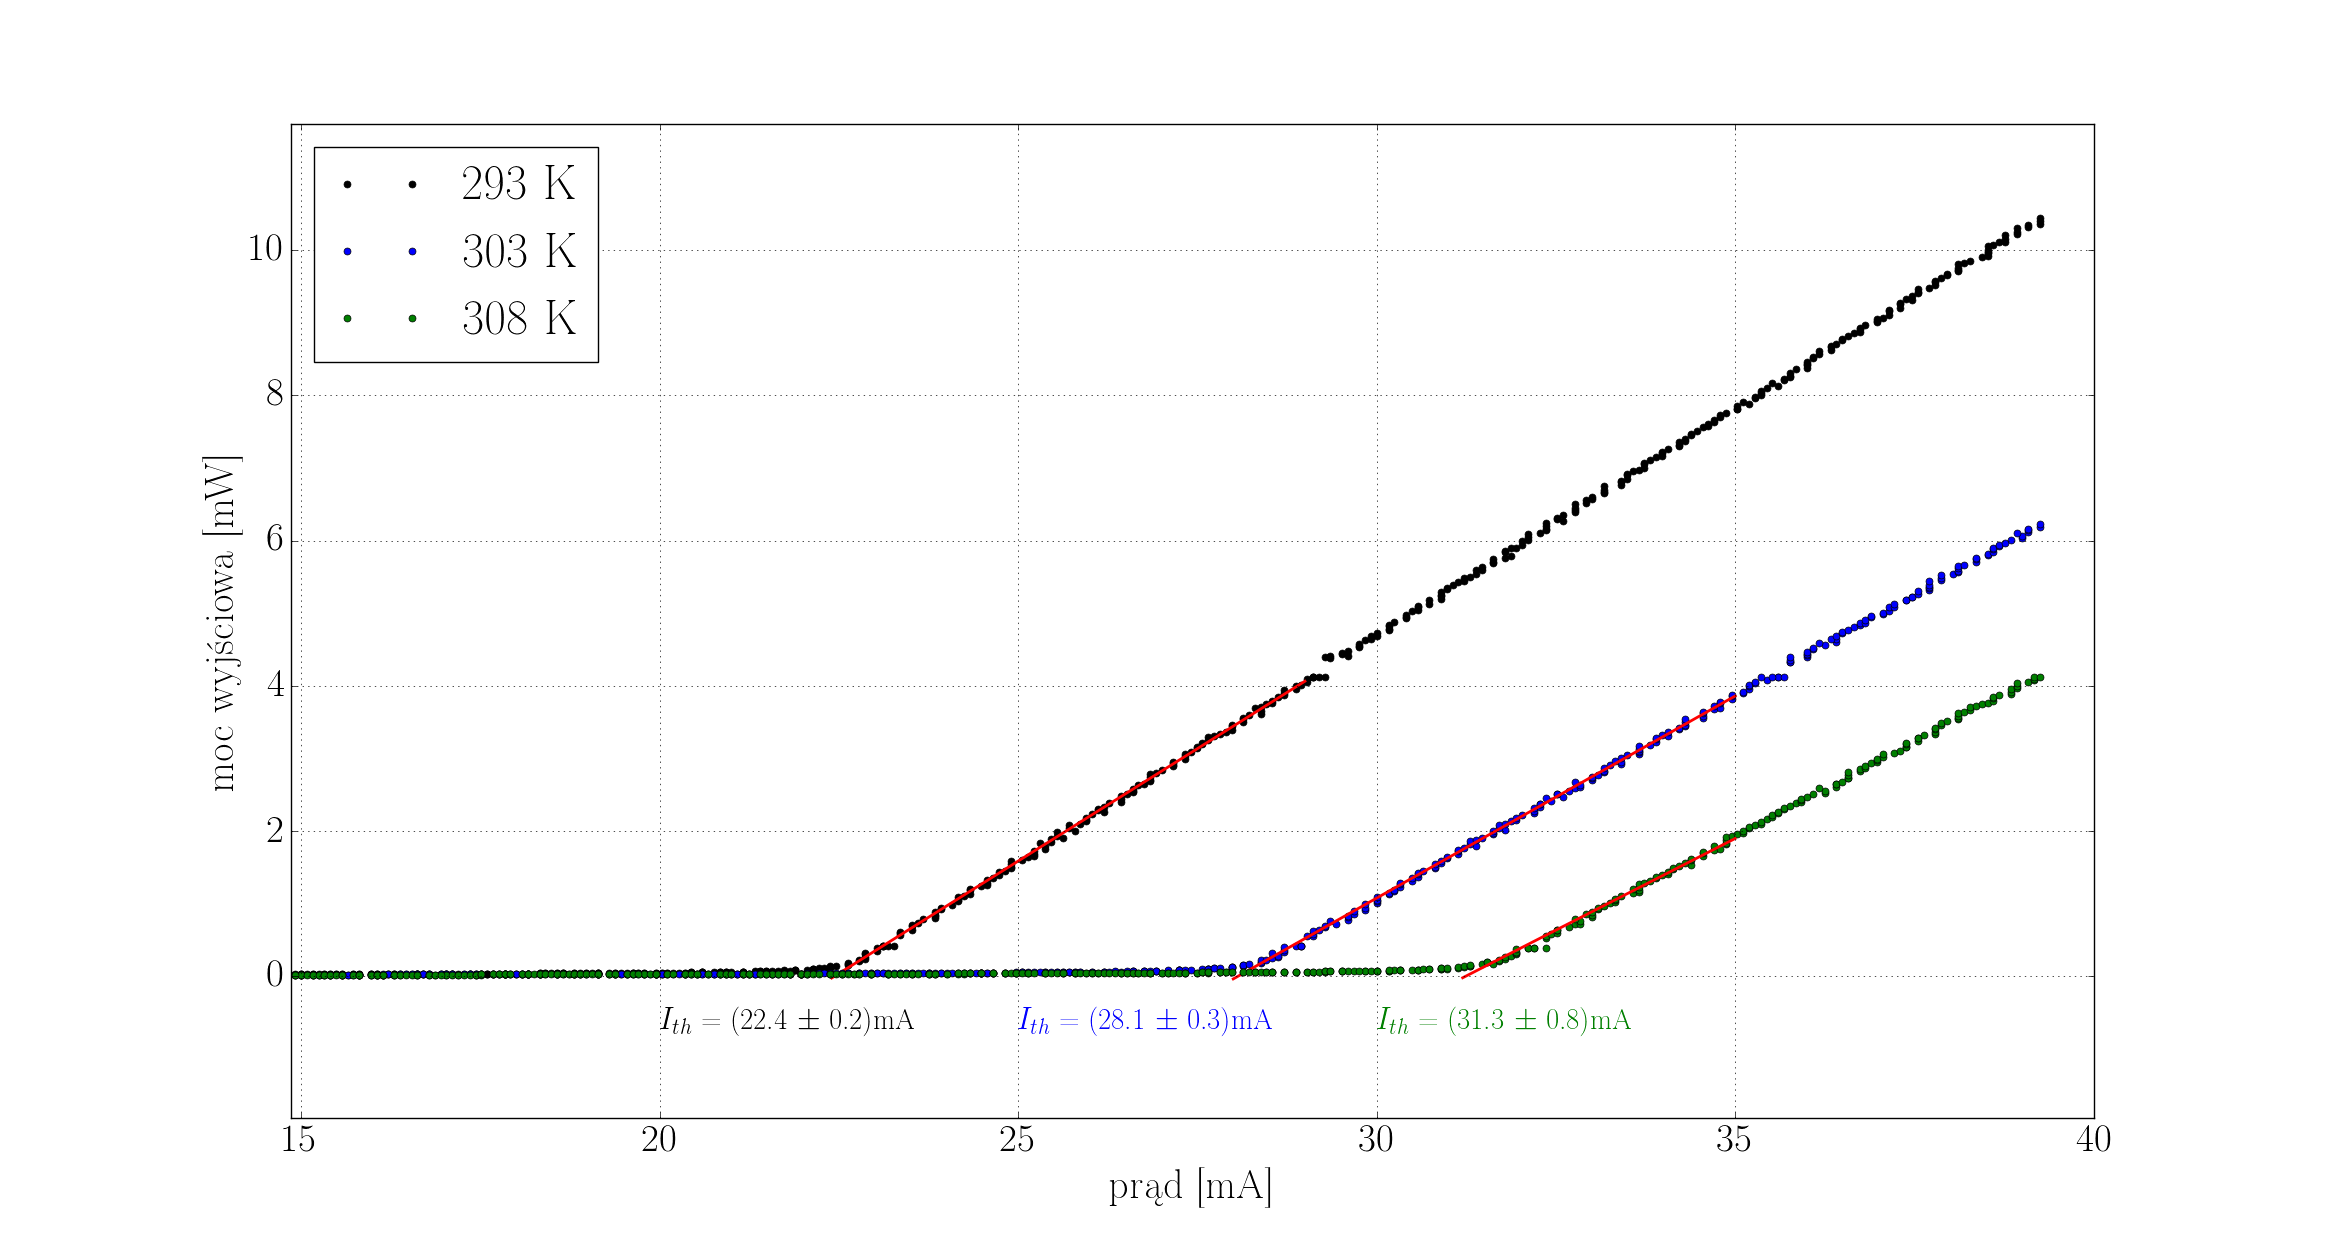
\includegraphics[scale=0.30]{plot635/plot_3_i_th.png}
  \label{rys1}
  \caption{Charakterystyka wyjściowej lasera krawędziowego 635 \,nm wraz z wyznaczonym prądem progowym dla różnych temperatur.} 
\end{figure}

\begin{figure}
\center
  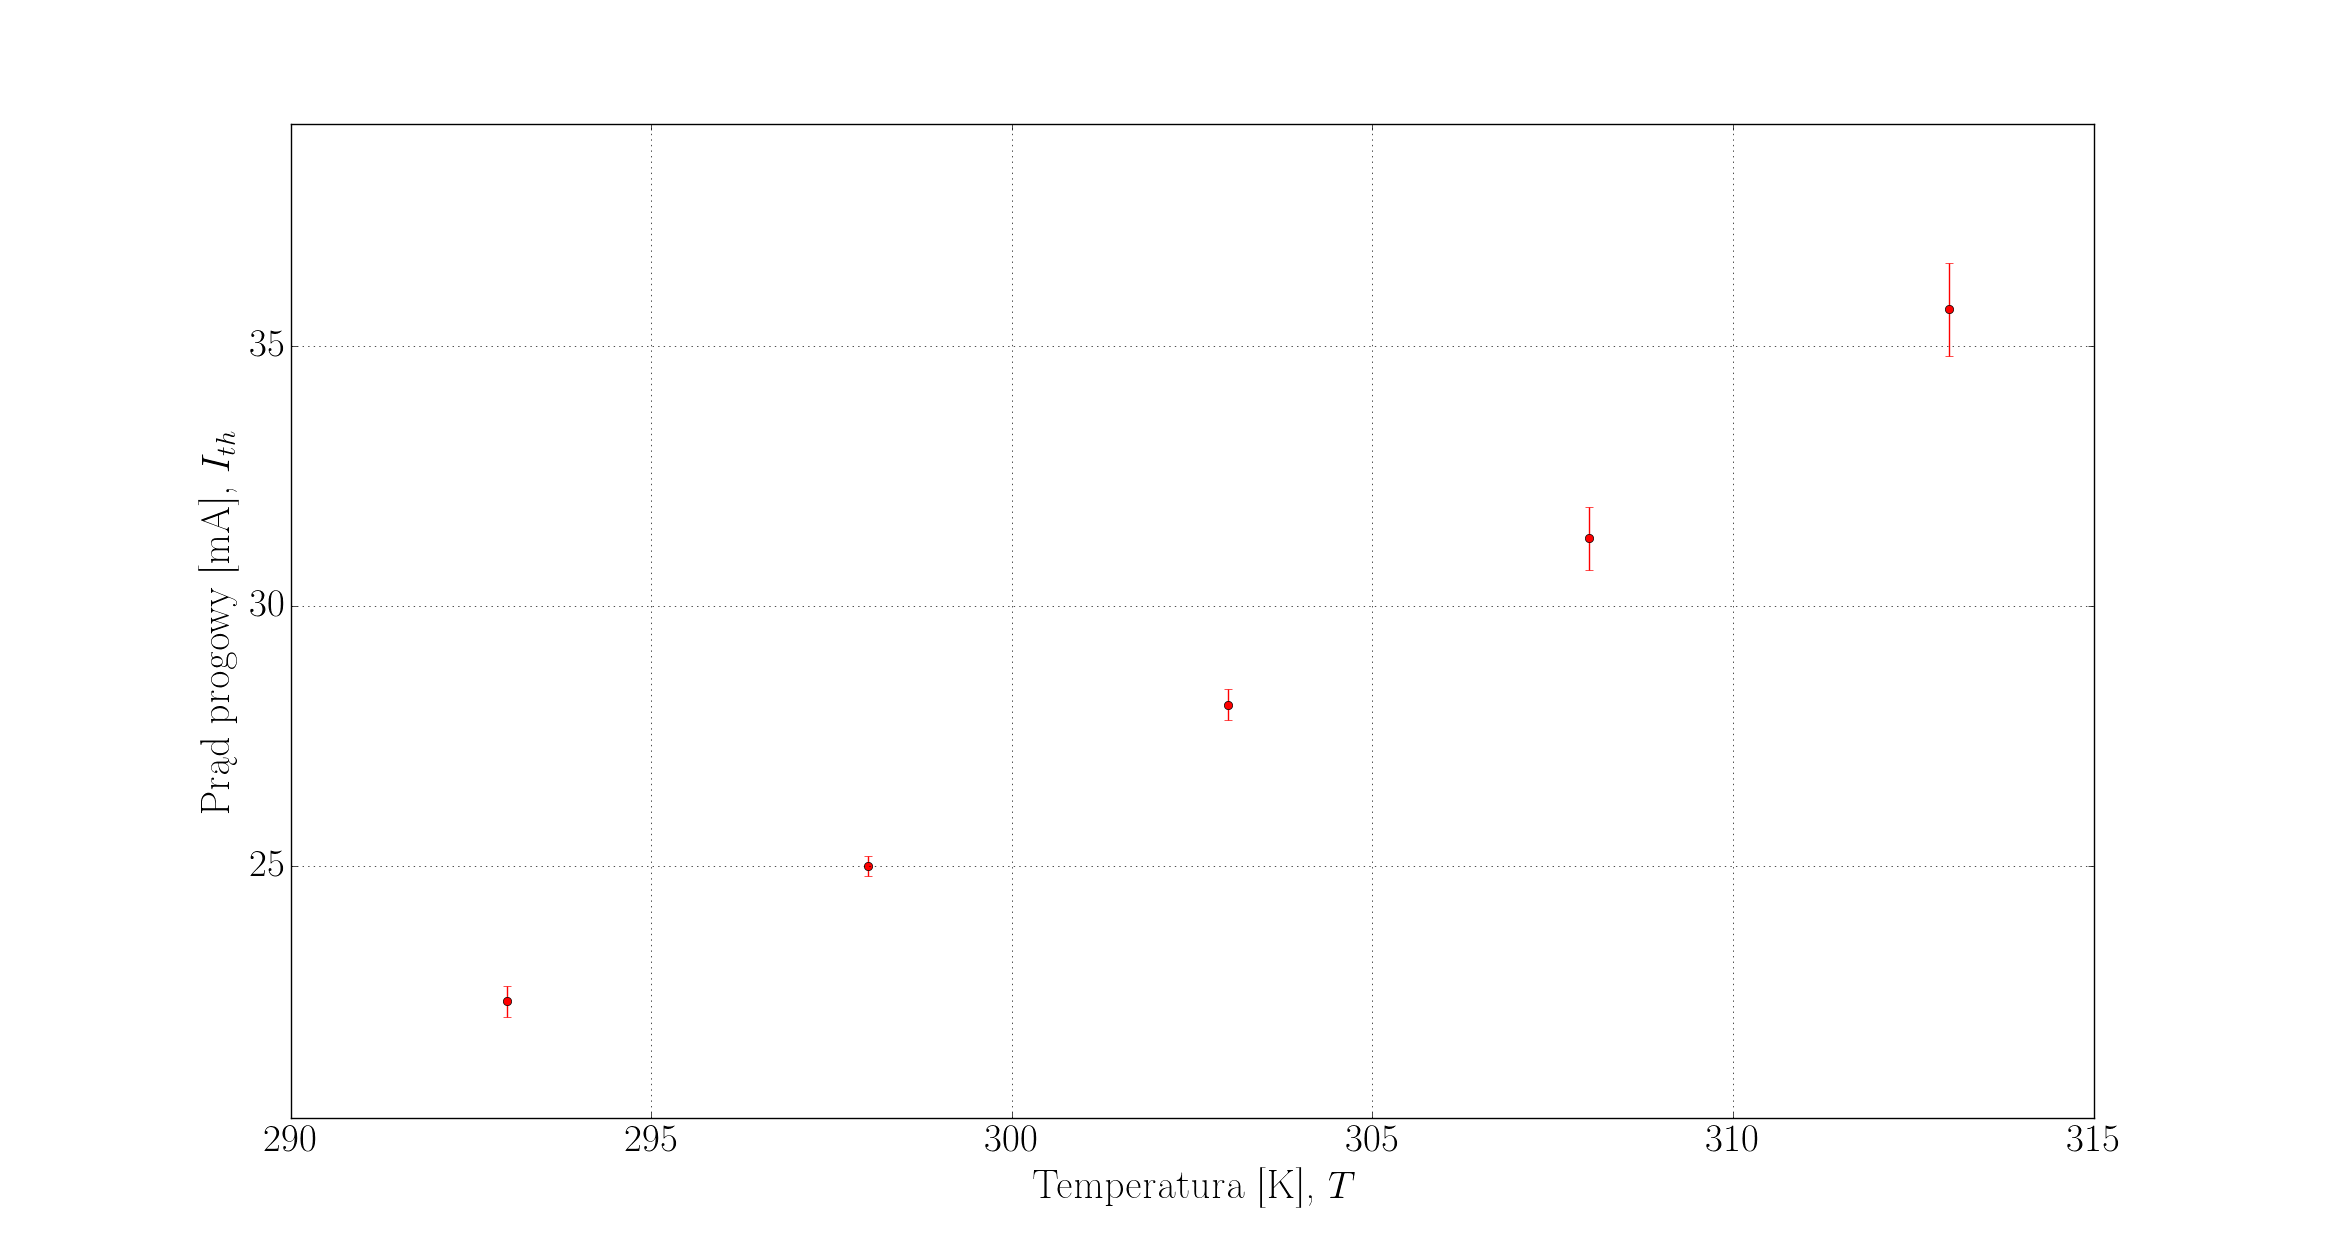
\includegraphics[scale=0.30]{plot635/plot_lin_i_th.png}
  \label{rys1}
  \caption{Wykres logarytmu z prądu progowego w zależności od temperatury chłodnicy wraz z wyznaczonymi parametrami $I_0$ i $T_0$ dla lasera krawędziowego 635 \,nm.} 
\end{figure}

\begin{figure}
\center
  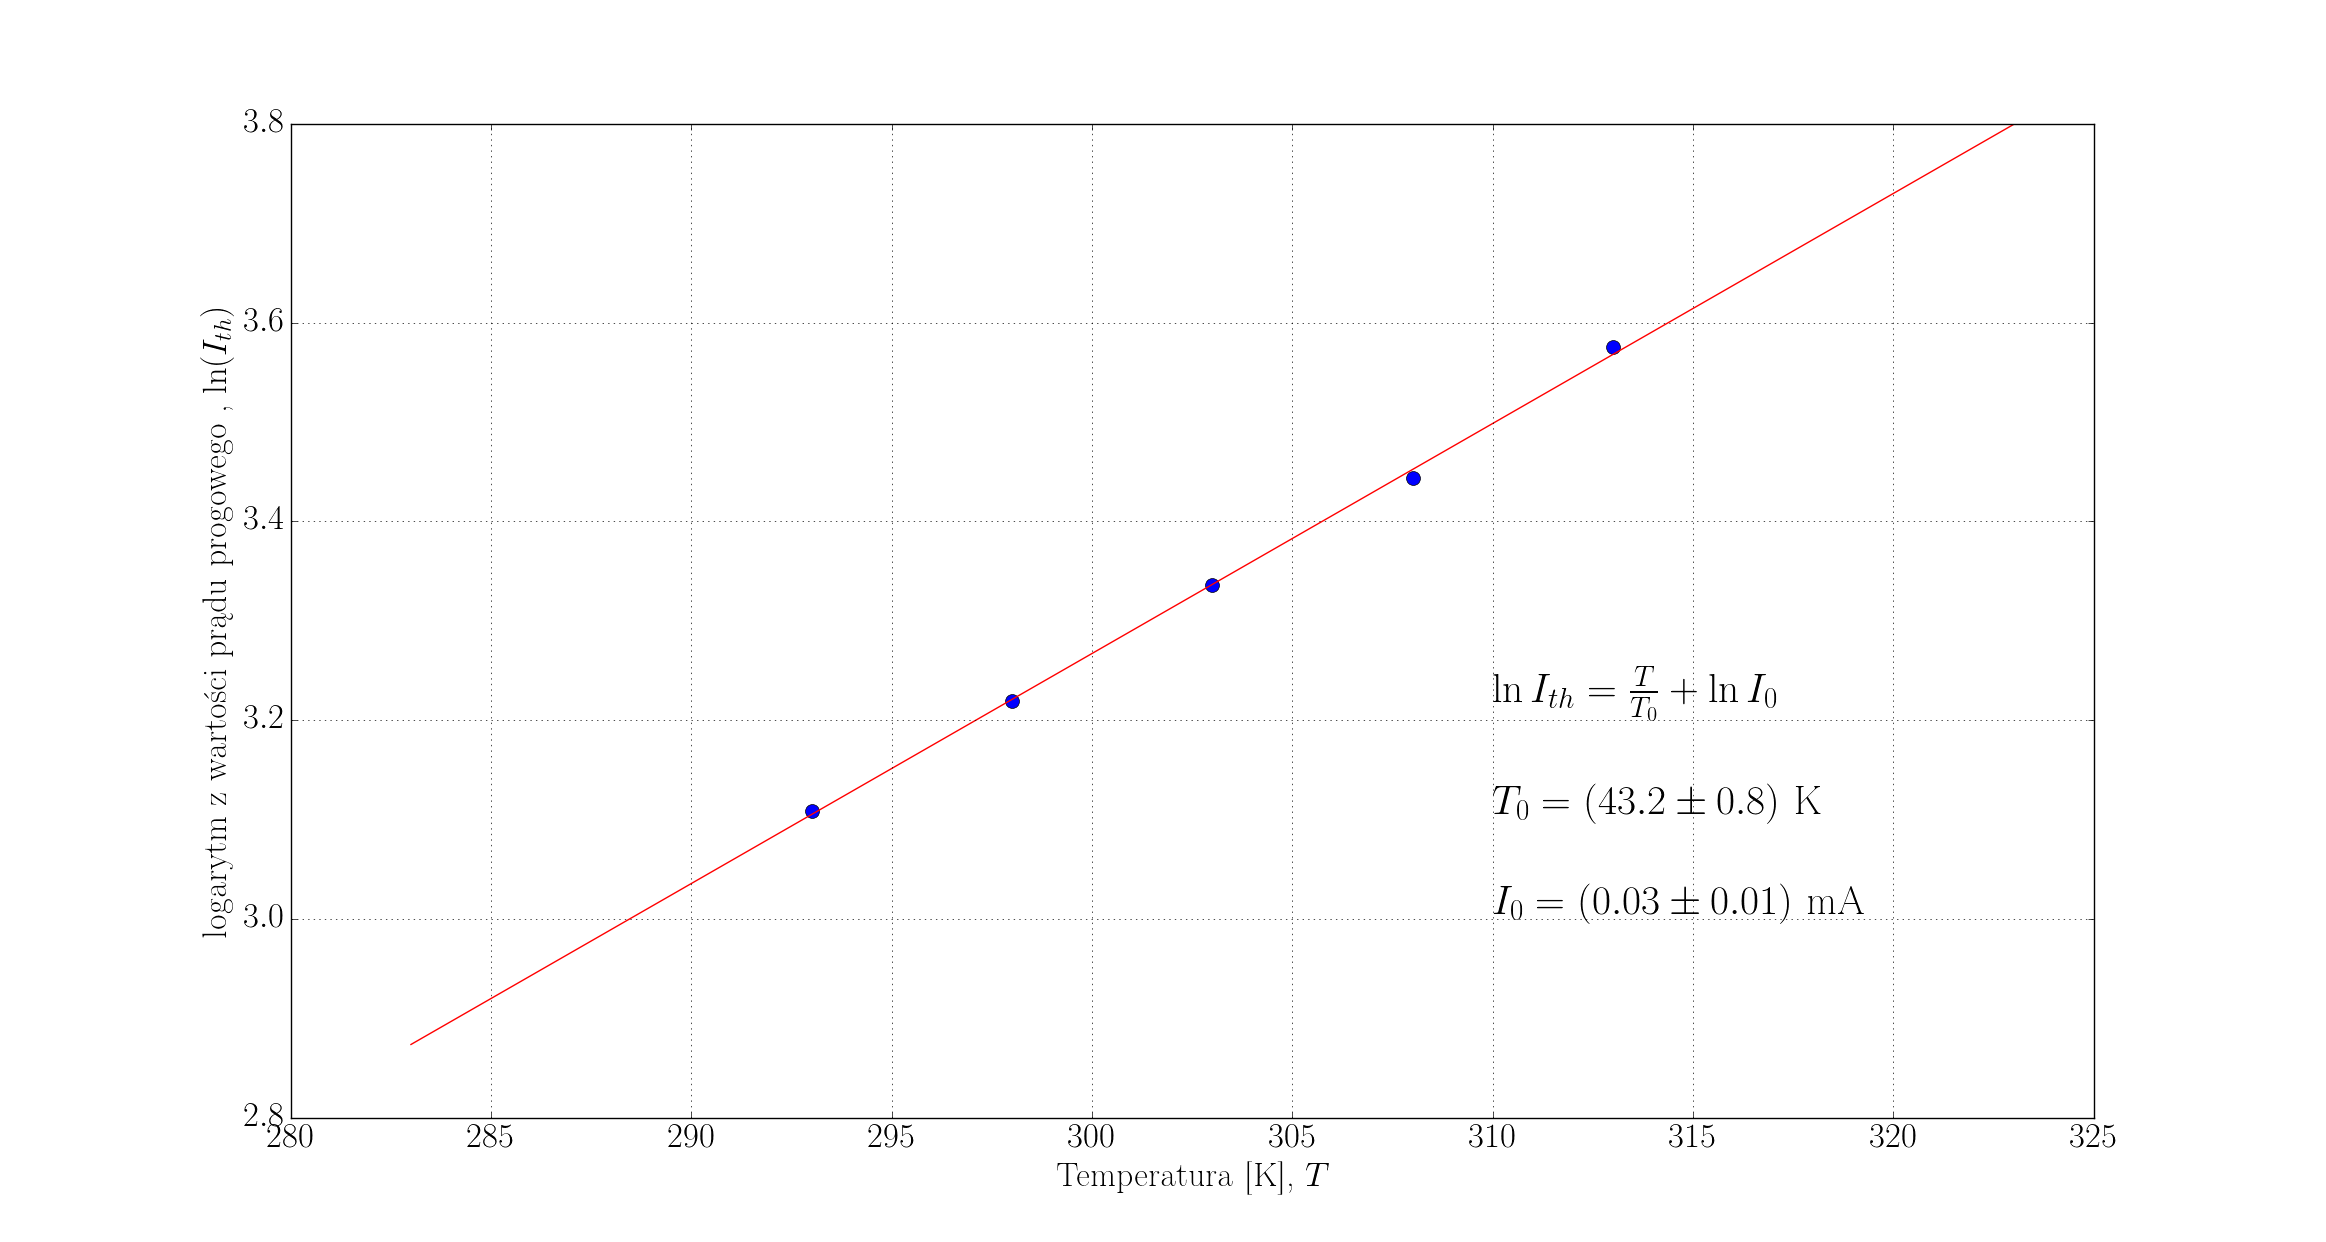
\includegraphics[scale=0.30]{plot635/fit_i_0.png}
  \label{rys1}
  \caption{Wykres logarytmu z prądu progowego w zależności od temperatury wraz z wyznaczonymi parametrami $I_0$ i $T_0$ dla lasera krawędziowego 635 \,nm.} 
\end{figure}



\end{document}